\documentclass[../main.tex]{subfiles}

\pagestyle{main}
\renewcommand{\chaptermark}[1]{\markboth{\chaptername\ \thechapter:\ #1}{}}
\setcounter{chapter}{15}

\begin{document}




\chapter{Multiple Integrals}
\section{Double Integrals}
\begin{itemize}
    \item \marginnote{12/19:}\textbf{Double integral} (of $F(x,y)$ over the region $A$): The limit as $\Delta A\to 0$ of the sum of every $\Delta A_k$ (composing $A$) times $F(x,y)$ for some $(x,y)\in\Delta A_k$. Mathematically,
    \begin{equation*}
        \int_A\int F(x,y)\dd{A} = \lim_{\Delta A\to 0}\sum_{k=1}^nF(x_k,y_k)\, \Delta A_k
    \end{equation*}
    \begin{figure}[h!]
        \centering
        \begin{subfigure}[b]{0.4\linewidth}
            \centering
            \begin{tikzpicture}[
                every node/.append style={black}
            ]
                \footnotesize
                \draw [->] (-0.4,0) -- (5,0) node[right]{$x$};
                \draw [->] (0,-0.4) -- (0,4) node[above]{$y$};
                \foreach \x/\name in {0.5/a,4.5/b} {
                    \draw (\x,0.1) -- ++(0,-0.2) node[below]{$\name$};
                }
                \node [anchor=north east] {$O$};

                \fill [ylz] (2,1.5) rectangle (2.5,2);
                \draw [very thin] (0.2,0.6) grid[step=5mm] (4.7,3.7);
                \node at (2.25,2.2) {$\Delta x$};
                \node [text height=1.5ex,text depth=0.25ex] at (1.76,1.75) {$\Delta y$};

                \draw [ylx,thick,name path=f1] (0.3,1.2) to[out=-45,in=180] (1.8,0.8) to[out=0,in=-150,out looseness=0.3] node[pos=0.4,below right,fill=white,inner sep=1.5pt]{$y=f_1(x)$} (4.7,1.6);
                \draw [ylx,thick,name path=f2] (0.3,2.8) to[out=45,in=180] (1.8,3.2) to[out=0,in=150,out looseness=0.3] node[pos=0.4,above right,fill=white,inner sep=1.5pt]{$y=f_2(x)$} (4.7,2.4);
                \draw [ylx,semithick,name path=a] (0.5,3.7) -- (0.5,0.6);
                \draw [ylx,semithick,name path=b] (4.5,3.7) -- (4.5,0.6);

                \begin{scope}[on background layer]
                    \fill [
                        gay,
                        name intersections={of=f1 and a,by={f1a}},
                        name intersections={of=f1 and b,by={f1b}},
                        name intersections={of=f2 and b,by={f2b}},
                        name intersections={of=f2 and a,by={f2a}}
                    ] (f1a) to[out=-30,in=180] (1.8,0.8) to[out=0,in=-153,out looseness=0.3] (f1b) -- (f2b) to[out=153,in=0,in looseness=0.3] (1.8,3.2) to[out=180,in=30] (f2a);
                \end{scope}
            \end{tikzpicture}
            \caption{Subdividing the region $A$.}
            \label{fig:doubleIntegrala}
        \end{subfigure}
        \begin{subfigure}[b]{0.4\linewidth}
            \centering
            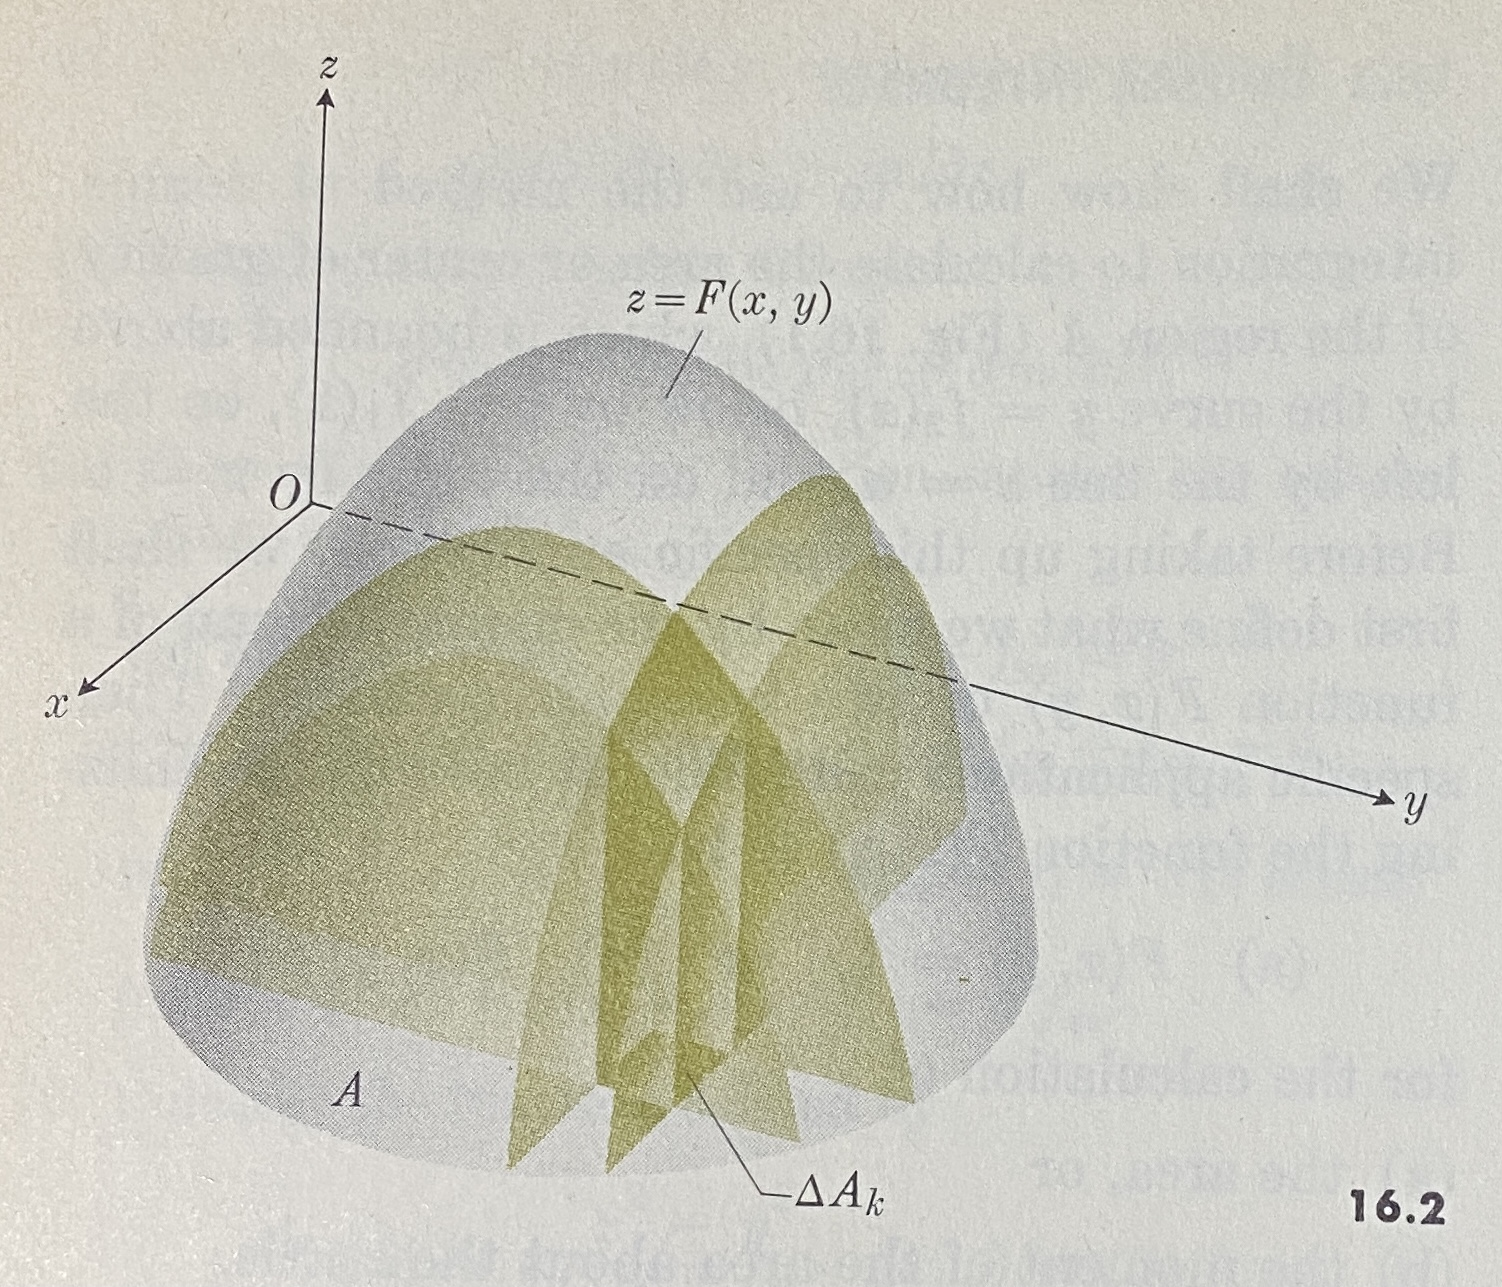
\includegraphics[width=0.9\linewidth]{ExtFiles/doubleIntegralb.jpg}
            \caption{Parts of $F(x,y)$ over a $\Delta A_k$.}
            \label{fig:doubleIntegralb}
        \end{subfigure}
        \caption{The double integral.}
        \label{fig:doubleIntegral}
    \end{figure}
    \begin{itemize}
        \item To conceptualize the double integral, first imagine that a region $A$ of the plane is bounded above by the curve $y=f_2(x)$, below by the curve $y=f_1(x)$, on the left by the line $x=a$, and on the right by the line $x=b$ (see Figure \ref{fig:doubleIntegrala}).
        \item Now imagine that $A$ is subdivided by a grid into $n$ pieces $\Delta A=\Delta x\Delta y=\Delta y\Delta x$. We disregard the pieces that lie partially or entirely outside of the bounds.
        \item As discussed in Chapter \ref{cht:15}, $F(x,y)$ can be thought of as a surface in three-space. For the sake of simplicity, we will imagine for right now that $F(x,y)$ is positive for all $(x,y)\in A$, i.e., that it lies above $A$ (see Figure \ref{fig:doubleIntegralb}).
        \item With this picture, we can imagine summing the partial volumes $F(x,y)\cdot\Delta A_k$ for each $\Delta A_k$ where $(x,y)$ is some point in $\Delta A_k$ to approximate the total volume under the surface (analogous to the area under the curve).
        \item All that the double integral does at this point is find the exact volume under the surface by taking the limit of this summation as we consider increasingly more increasingly small slivers of volume.
    \end{itemize}
    \item We can evaluate the double integral of $F(x,y)$ over $A$ if $F(x,y)$ is continuous throughout $A$, if the boundary curves are continuous and have finite total length, and if we let $\Delta y=2\Delta x$ (or some other similar function) and let $\Delta x\to 0$.
    \item To evaluate double integrals, we calculate one or the other of the \textbf{iterated} integrals\footnote{Proving that evaluating these integrals is equivalent to evaluating the double integral is a more advanced theorem of analysis.}
    \begin{align*}
        \int_A\int F(x,y)\dd{x}\dd{y}&&
            \int_A\int F(x,y)\dd{y}\dd{x}
    \end{align*}
    \item To evaluate the latter integral above, for example, we integrate \dq{$\int F(x,y)\dd{y}$ with respect to $y$ (with $x$ held fixed) and [evaluate] the resulting integral between the limits $y=f_1(x)$ and $y=f_2(x)$, and then [integrate] the result\dots with respect to $x$ between the limits $x=a$ and $x=b$}{549} Mathematically,
    \begin{equation*}
        \int_A\int F(x,y)\dd{y}\dd{x} = \int_a^b\left( \int_{f_1(x)}^{f_2(x)}F(x,y)\dd{y} \right)\dd{x}
    \end{equation*}
    \begin{figure}[h!]
        \centering
        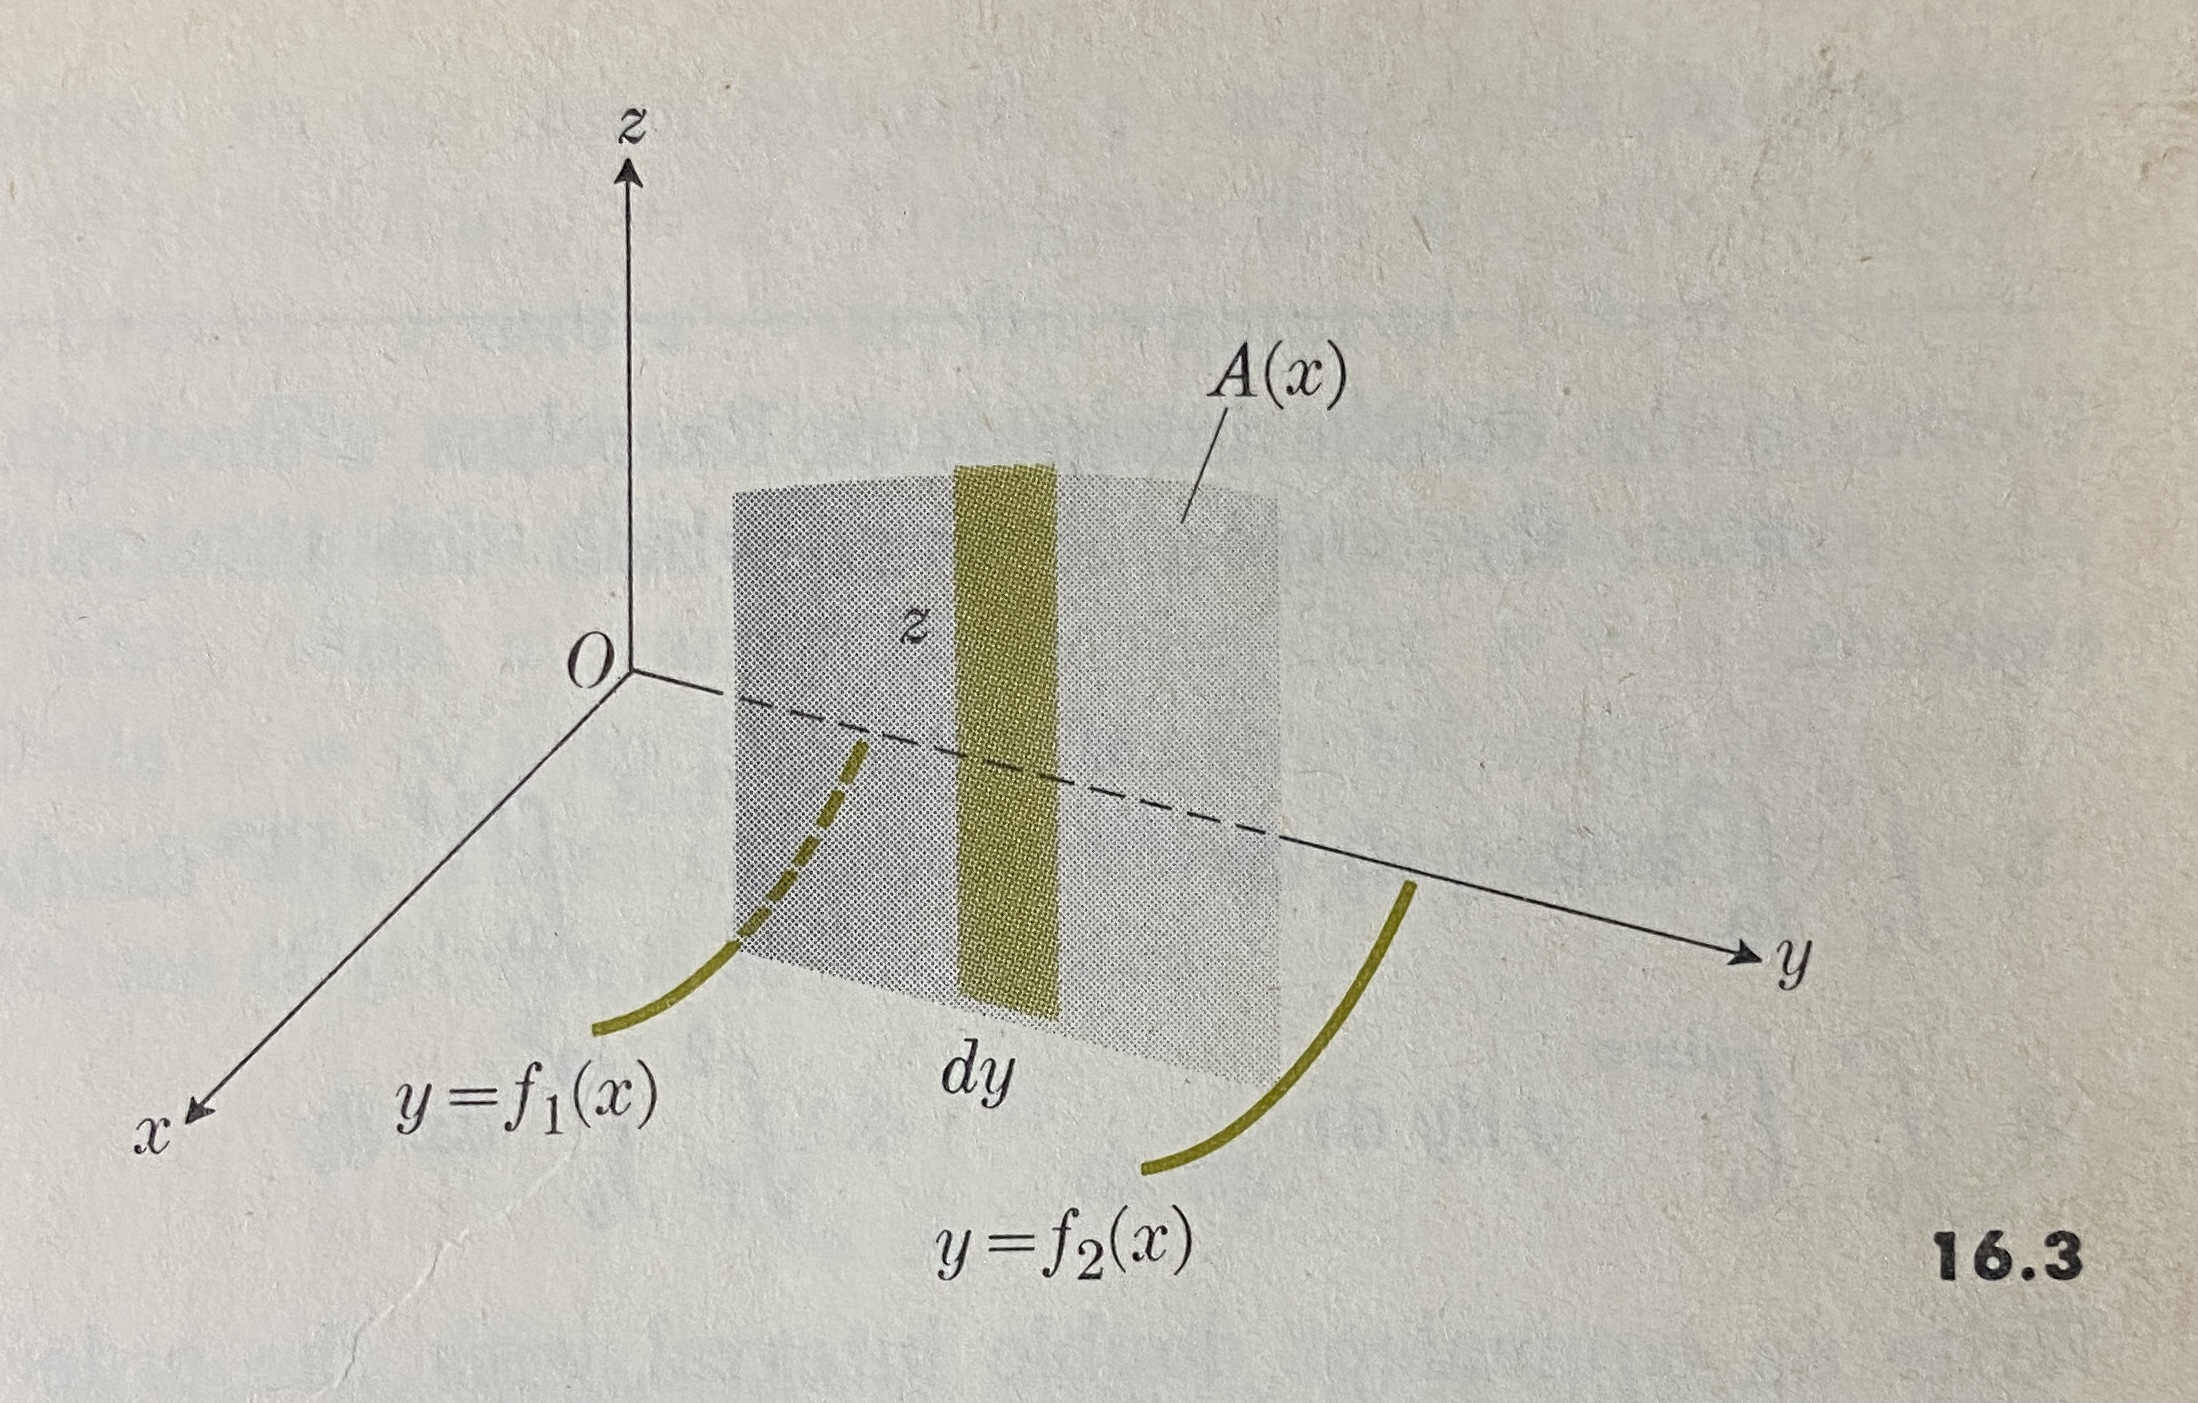
\includegraphics[width=0.4\linewidth]{ExtFiles/interatedIntegration.jpg}
        \caption{Visualizing iterated integration.}
        \label{fig:iteratedIntegration}
    \end{figure}
    \begin{itemize}
        \item To visualize iterated integration, imagine determining the volume under the surface by summing infinitely many infinitely thin cross sections of the solid parallel to the $y$-axis.
        \item The cross section at $x=x_0$ would have area $A(x_0)=\int_{f_1(x_0)}^{f_2(x_0)} F(x_0,y)\dd{y}$.
        \item The sum of all such cross sections' contributions to the volume would be the integral $\int_a^bA(x)\dd{x}=\int_a^b\left( \int_{f_1(x)}^{f_2(x)} F(x,y)\dd{y} \right)\dd{x}$.
    \end{itemize}
\end{itemize}



\section{Area by Double Integration}
\begin{itemize}
    \item The area of the region of the $xy$-plane is given by either of the following integrals (with proper limits of integration).
    \begin{equation*}
        A = \iint\dd{x}\dd{y} = \iint\dd{y}\dd{x}
    \end{equation*}
    \item In cases such as that of Figure \ref{fig:doubleIntegrala}, it makes sense to integrate with respect to $y$ first and $x$ second. However, if we have a region bounded by $y=c$, $y=d$, $x=g_1(y)$, and $x=g_2(y)$, then it would make more sense to do the opposite.
    \item Conceptualize the iterated integration here as summing the infinitesimal areas of strips parallel to the $x$- or $y$-axis, the lengths of which are given by $f_2(x)-f_1(x)=\int_{f_1(x)}^{f_2(x)}\dd{y}$ or $g_2(y)-g_1(y)=\int_{g_1(y)}^{g_2(y)}\dd{x}$.
\end{itemize}



\section{Physical Applications}
\begin{figure}[h!]\marginnote{12/20:}
    \centering
    \begin{tikzpicture}[
        every node/.append style={black}
    ]
        \footnotesize
        \draw [->] (-0.5,0) -- (5,0) node[right]{$x$};
        \draw [->] (0,-0.4) -- (0,3.5) node[above]{$y$};
        \node [anchor=north east] {$O$};

        \filldraw [fill=gay,draw=ylx,thick] (3.5,0.5)
            to[out=0,in=-90] (4.5,1.2)
            to[out=90,in=0] (1.5,2.8)
            to[out=180,in=90] (0.3,1.7)
            to[out=-90,in=180] (1,0.7)
            to[out=0,in=180] (2,0.8)
            to[out=0,in=180] cycle
        ;
        \node at (3.5,1.8) {$A$};
        \fill [ylz] (2,1.5) -- node[above]{$\dd{A}$} node[below]{$\dd{x}$} ++(0.5,0) -- ++(0,0.5) -- ++(-0.5,0) -- node[left]{$\dd{y}$} cycle;
    \end{tikzpicture}
    \caption{A planar mass.}
    \label{fig:planarMass}
\end{figure}
\begin{itemize}
    \item Imagine that there is a mass continuously distributed over a region $A$ in the $xy$-plane, where the 2D density at every point $(x,y)\in A$ is given by $\delta(x,y)$.
    \item It follows that $\dd{m}=\delta(x,y)\dd{A}$, so the mass, the first moment of the mass with respect to the $x$-axis, and the first moment of the mass with respect to the $y$-axis are, respectively,
    \begin{align*}
        M &= \iint\delta(x,y)\dd{A}&
            M_x &= \iint y\, \delta(x,y)\dd{A}&
                M_y &= \iint x\, \delta(x,y)\dd{A}
    \end{align*}
    \item From these equations, we can also get the coordinates of the center of mass:
    \begin{equation*}
        (x_\text{cm},y_\text{cm}) = \left( \frac{M_y}{M},\frac{M_x}{M} \right)
    \end{equation*}
    \item The moments of inertia (second moments of the mass) with respect to the $x$- and $y$-axes, and the polar moment of inertia about the origin are, respectively,
    \begin{align*}
        I_x &= \iint y^2\, \delta(x,y)\dd{A}&
            I_y &= \iint x^2\, \delta(x,y)\dd{A}&
                I_0 &= \iint r^2\, \delta(x,y)\dd{A}
    \end{align*}
    \item \cite{bib:Thomas} defines the moment of inertia from a physics perspective, including the formula
    \begin{equation*}
        I = \lim_{\Delta m\to 0}\sum r^2\, \Delta m = \int r^2\dd{m}
    \end{equation*}
    and then talks a bit about stiffness and why I-beams are strong.
    \item Statistical importance of moments:
    \begin{itemize}
        \item The first moment helps compute the mean $\bar{r}$:
        \begin{equation*}
            \bar{r} = \frac{\sum m_kr_k}{\sum m_k} = \frac{M_1}{M}
        \end{equation*}
        \item The second moment helps compute the variance $\sigma^2$ and standard deviation $\sigma$:
        \begin{equation*}
            \sigma^2 = \frac{\sum(r_k-\bar{r})^2m_k}{\sum m_k} = \frac{M_2}{M}-\bar{r}^2
        \end{equation*}
        \begin{itemize}
            \item Both $\sigma^2$ and $\sigma$ are \dq{measures of the way in which the $r$-values tend to bunch up close to $\bar{r}$ (small values of $\sigma$) or to be spread out (large values of $\sigma$)}{554}
        \end{itemize}
        \item The third moment helps compute the \textbf{skewness}.
        \item The fourth moment helps compute the \textbf{kurtosis}.
        \item The $t^\text{th}$ moment is defined as
        \begin{equation*}
            M_t = \sum_{k=1}^nm_kr_k^t
        \end{equation*}
        \begin{itemize}
            \item $r_k$ ranges over all values of the statistic under consideration, and $m_k$ is the number of times it occurs (e.g., if 5 students score a 75\% on a quiz, then $r_k=75$ and $m_k=5$ where a 75\% is the $k^\text{th}$ score earned).
        \end{itemize}
    \end{itemize}
    \item \textbf{Frequency distribution}: \dq{A table of values of $m_k$ versus $r_k$}{553}
    \begin{itemize}
        \item $M_t$ is \dq{the $t^\text{th}$ moment of this frequency distribution}{553}
    \end{itemize}
    \item Note that area integrals such as $A=\int_a^by\dd{x}$ require substituting for $y$ whereas double integrals do not, as we are integrating with respect to $y$ in part, and the boundary curves are only applied as limits of integration. In double integrals, the point $(x,y)$ is an element of $\dd{A}$, and $x,y$ are both independent variables.
    \item \textbf{Radius of gyration} (of an object of mass $M$ about an axis where the object has moment of inertia $I$): The number $\sqrt{I/M}$ representing the radius a radial point particle (a loop) with equal mass would have to have in order to have the same moment of inertia as the object at hand.
\end{itemize}



\section{Polar Coordinates}
\begin{itemize}
    \item \textbf{Double integral} (of $F(r,\theta)$ over the region $A$): The limit as $\Delta A\to 0$ of the sum of every $\Delta A_k$ (composing $A$) times $F(r_k,\theta_k)$ where $(r_k,\theta_k)$ is the point in the center\footnote{The intersection of the arc halfway between $r$ and $r+\Delta r$ and the ray halfway between $\theta$ and $\theta+\Delta\theta$.} of $\Delta A_k$. Mathematically,
    \begin{equation*}
        \int_A\int F(r,\theta)\dd{A} = \lim_{\Delta A\to 0}\sum_{k=1}^nF(r_k,\theta_k)\, \Delta A_k
    \end{equation*}
    \begin{figure}[h!]
        \centering
        \begin{tikzpicture}[
            every node/.append style={black},
            scale=1.15
        ]
            \footnotesize
            \draw [->] (-6,0) node[left]{$\theta=\pi$} -- node[below]{$O$} (6,0) node[right]{$\theta=0$};
            \draw (5,0) arc[start angle=0,end angle=180,radius=5cm];
            \node [right] at (15:5) {$r=a$};
            \foreach \r in {0.625,1.25,...,4.375} {
                \draw [very thin] (30:\r) arc[start angle=30,end angle=135,radius=\r];
            }
            \foreach \r/\n in {0.625/,1.25/2,1.875/3} {
                \node [left] at (135:\r) {$\n\Delta r$};
            }
            \foreach \thta in {30,45,...,135} {
                \draw [very thin] (0:0) -- (\thta:5);
            }
            \foreach \thta/\n in {45/,60/2} {
                \node [above right=-2pt] at (\thta:5) {$\alpha+\n\Delta\theta$};
            }

            \draw [ylx,semithick] (0:0) -- node[pos=0.92,below right=-2pt]{$\theta=\alpha$} (30:5.8);
            \draw [ylx,semithick] (0:0) -- node[pos=0.92,below left=-2pt]{$\theta=\beta$} (135:5.8);
            \draw [ylx,thick] (30:2.45) node[below right=-2pt]{$r=f_1(\theta)$}
                to[out=150,in=0] (50:2)
                to[out=180,in=0] (90:1.5)
                to[out=180,in=-10] (135:2.25)
            ;
            \draw [ylx,thick] (30:3.5) node[below right=-2pt]{$r=f_2(\theta)$}
                to[out=110,in=0,in looseness=0.7] (90:4.75)
                to[out=180,in=50,out looseness=0.8] (135:4.125)
            ;

            \begin{scope}[on background layer]
                \fill [gay] (0:0) -- (30:5) arc[start angle=30,end angle=135,radius=5cm];
                \fill [ylz] (75:3.75) arc (75:90:3.75) -- (90:3.125) arc (90:75:3.125) -- node[pos=0.4,right]{$\Delta r$} cycle;
                \fill (82.5:3.4375) circle (1.5pt);
                \node [inner sep=0pt] at (97.5:3.4375) {$(r_k,\theta_k)$}
                    edge (82.5:3.4375)
                ;
                \node [inner sep=0pt] at (82.5:4) {$\Delta A_k$}
                    edge (82.5:3.6)
                ;
                \coordinate (O) at (0,0);
                \coordinate (X) at (75:5);
                \coordinate (Y) at (90:5);
                \pic [draw,->,angle radius=3.25cm,pic text={$\Delta\theta$},angle eccentricity=0.94] {angle=X--O--Y};
            \end{scope}
        \end{tikzpicture}
        \caption{The double integral in polar coordinates.}
        \label{fig:polarDoubleIntegrals}
    \end{figure}
    \item If we subdivide $A$ as in Figure \ref{fig:polarDoubleIntegrals}, we find that
    \begin{align*}
        \Delta A_k &= \frac{1}{2}\left( r_k+\frac{1}{2}\Delta r \right)^2\Delta\theta-\frac{1}{2}\left( r_k-\frac{1}{2}\Delta r \right)^2\Delta\theta\\
        &= r_k\, \Delta\theta\, \Delta r
    \end{align*}
    \item Therefore, to evaluate the double integral of $F(r,\theta)$ over the region $A$, we calculate the iterated integral on the right below.
    \begin{equation*}
        \int_A\int F(r,\theta)\dd{A} = \int_{\theta=\alpha}^\beta\int_{r=f_1(\theta)}^{f_2(\theta)}F(r,\theta)\, r\dd{r}\dd{\theta}
    \end{equation*}
    \item To change from $xy$- to $uv$- coordinates in a double integral, where we integrate over a region $A$ in the $xy$-plane that is equivalent to the region $G$ in the $uv$-plane and have $x=f(u,v),y=g(u,v)$, use the formula
    \begin{equation*}
        \int_A\int\phi(x,y)\dd{x}\dd{y} = \int_G\int\phi[f(u,v),g(u,v)]\pdv{(x,y)}{(u,v)}\dd{u}\dd{v}
    \end{equation*}
    where
    \begin{equation*}
        \renewcommand{\arraystretch}{1.6}
        \pdv{(x,y)}{(u,v)} =
        \begin{vmatrix}
            \pdv{x}{u} & \pdv{x}{v}\\
            \pdv{y}{u} & \pdv{y}{v}\\
        \end{vmatrix}
    \end{equation*}
    is the \textbf{Jacobian} of the transformation.
    \item For example, to switch from $xy$- to polar coordinates, we have $x=r\cos\theta$, $y=r\sin\theta$ and
    \begin{equation*}
        \renewcommand{\arraystretch}{1.6}
        \pdv{(x,y)}{(r,\theta)} =
        \begin{vmatrix}
            \pdv{x}{r} & \pdv{x}{\theta}\\
            \pdv{y}{r} & \pdv{y}{\theta}\\
        \end{vmatrix}
        =
        \begin{vmatrix}
            \cos\theta & -r\sin\theta\\
            \sin\theta & r\cos\theta\\
        \end{vmatrix}
        = r(\cos^2\theta+\sin^2\theta)
        = r
    \end{equation*}
    so we get
    \begin{equation*}
        \iint\phi(x,y)\dd{x}\dd{y} = \iint\phi(r\cos\theta,r\sin\theta)\, r\dd{r}\dd{\theta}
    \end{equation*}
\end{itemize}



\section{Triple Integrals: Volume}
\begin{itemize}
    \item \textbf{Riemann triple integral} (of $F(x,y,z)$ over $V$): The limit as $\Delta V\to 0$ of the sum of every $\Delta V_k$ (composing $V$) times $F(x,y,z)$ for some point $(x,y,z)\in \Delta V_k$. Mathematically,
    \begin{equation*}
        \iiint\limits_VF(x,y,z)\dd{V} = \lim_{\Delta V\to 0}\sum_{k=1}^nF(x_k,y_k,z_k)\, \Delta V_k
    \end{equation*}
    \item Some interpretations of the triple integral:
    \begin{itemize}
        \item $F(x,y,z)=1$: The volume of $V$.
        \item $F(x,y,z)=x$: The first moment of the volume $V$ with respect to the $yz$-plane.
        \item $F(x,y,z)$ is the density at $(x,y,z)$: The mass in $V$.
        \item $F(x,y,z)$ is "the product of the density at $(x,y,z)$ and the square of the distance from $(x,y,z)$ to an axis $L$" \parencite[558]{bib:Thomas}: The moment of inertia of the mass with respect to $L$.
    \end{itemize}
    \item To evaluate triple integrals, we calculate an iterated integral of the following form, where $f_1(x,y)$ and $f_2(x,y)$ are surfaces that enclose $V$ on the top and bottom, and $A$ is the region of the $xy$-plane enclosed by the cylinder $C$ that bounds $V$ laterally with elements parallel to the $z$-axis.
    \begin{equation*}
        \int_A\iint_{f_1(x,y)}^{f_2(x,y)}F(x,y,z)\dd{z}\dd{y}\dd{x}
    \end{equation*}
    \begin{figure}[h!]
        \centering
        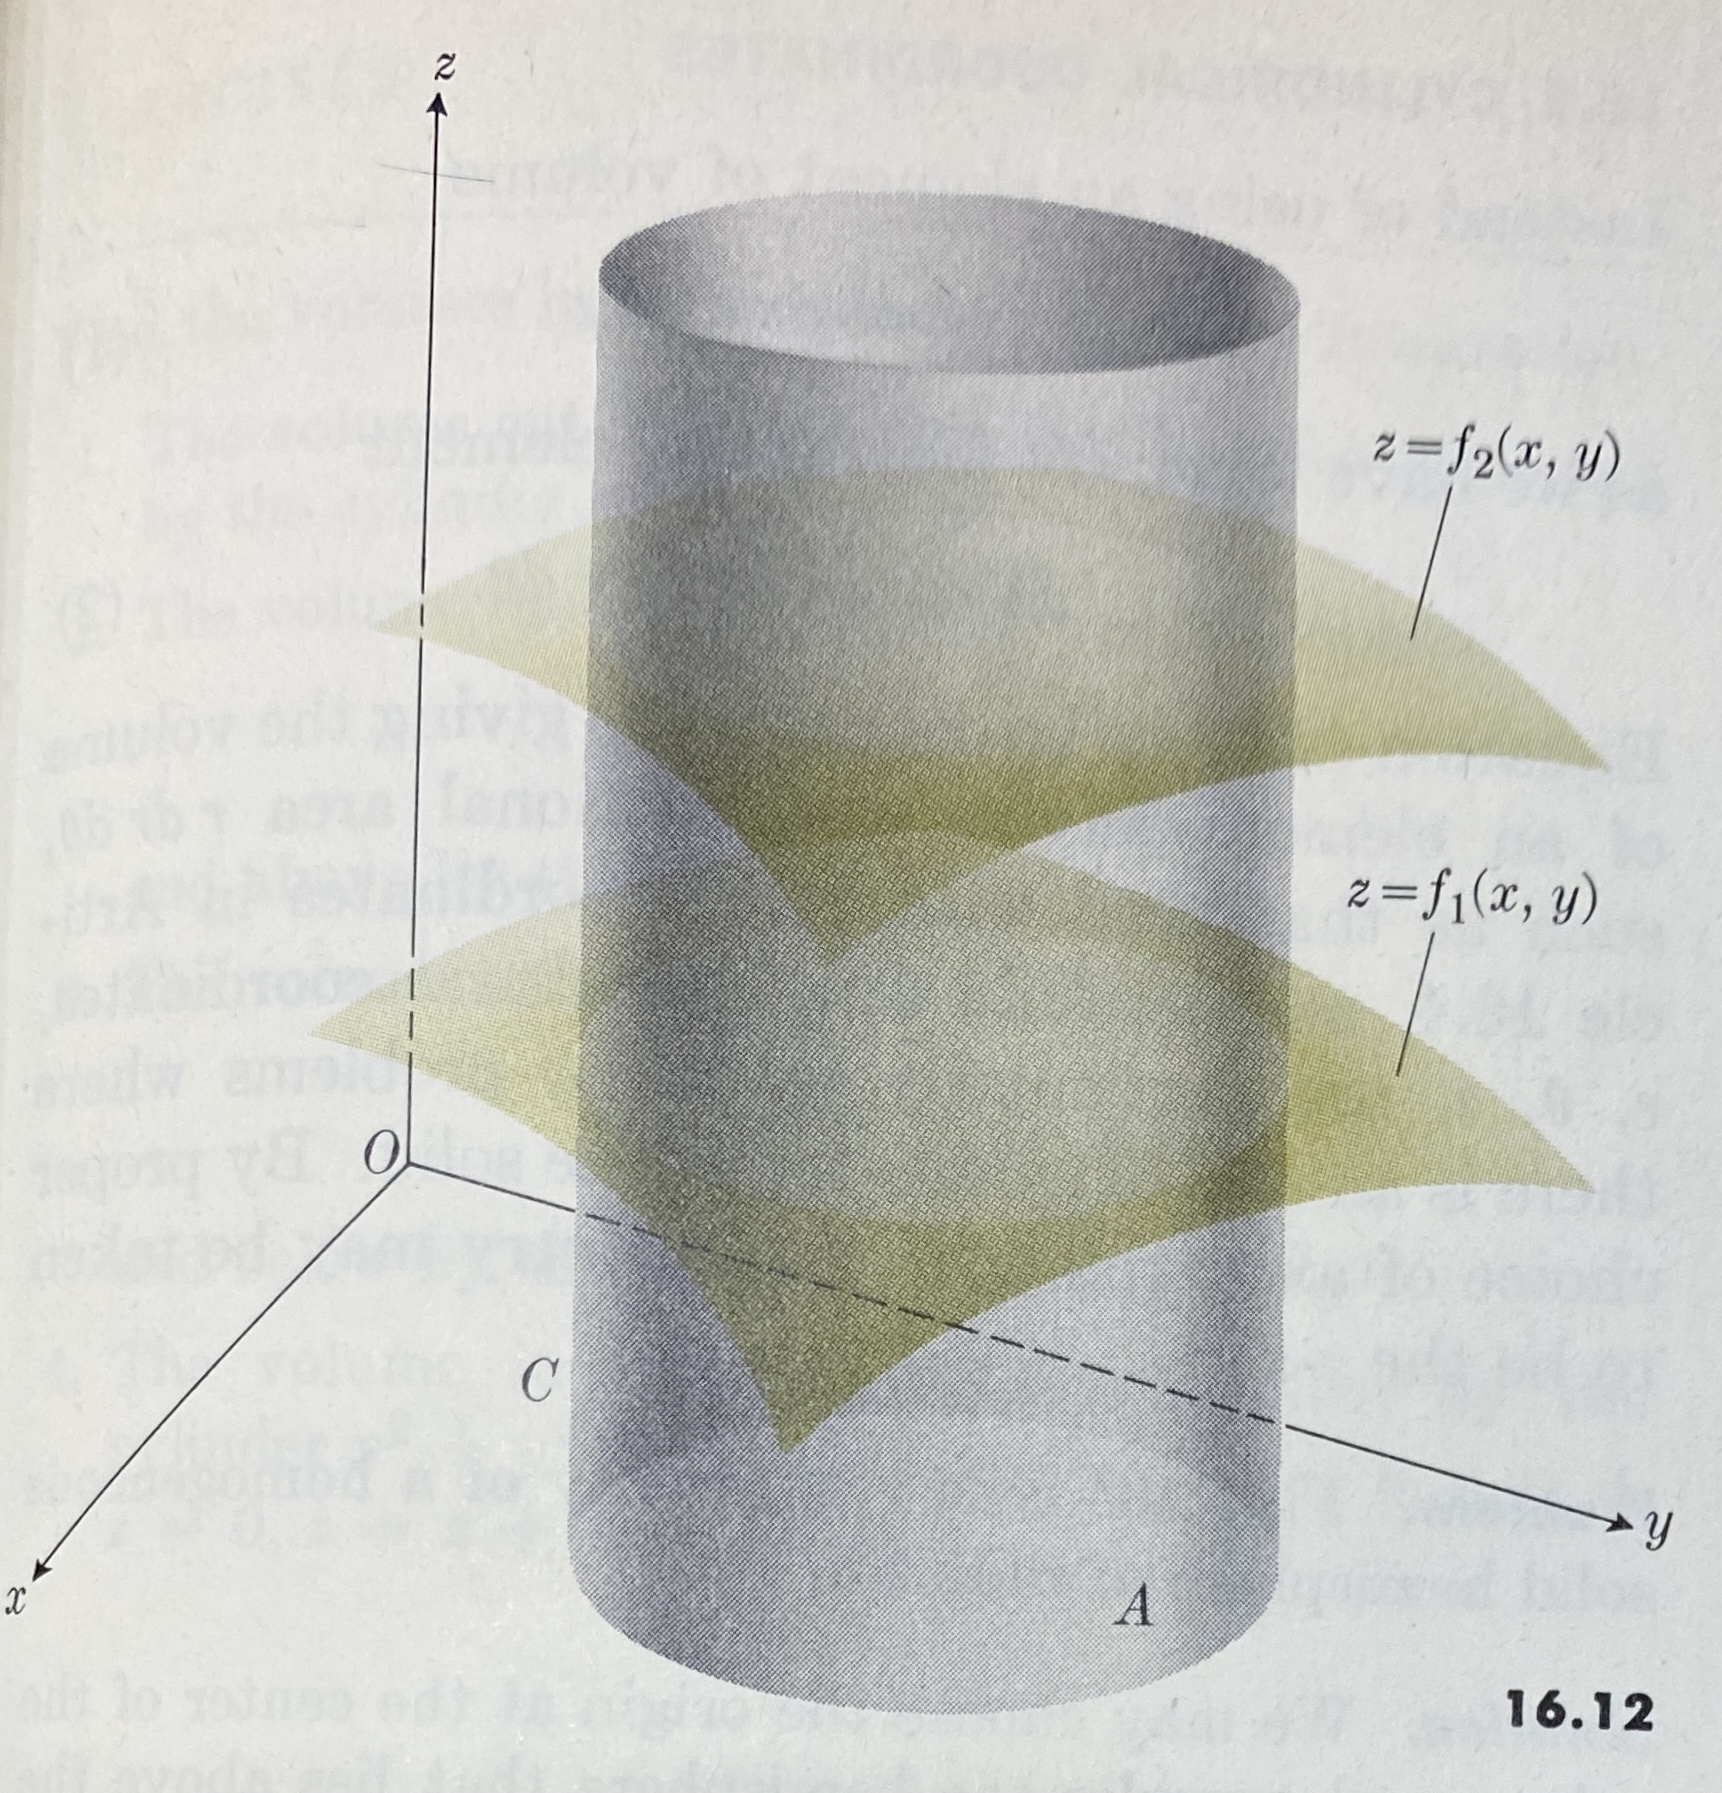
\includegraphics[width=0.4\linewidth]{ExtFiles/tripleIntegral.jpg}
        \caption{The triple integral.}
        \label{fig:tripleIntegral}
    \end{figure}
    \begin{itemize}
        \item The first integral is a normal integral with $x,y$ held constant, and the second one is a double integral over $A$.
    \end{itemize}
    \item \dq{Find the volume enclosed between the two surfaces $z=8-x^2-y^2$ and $z=x^2+3y^2$}{559}
    \begin{figure}[H]
        \centering
        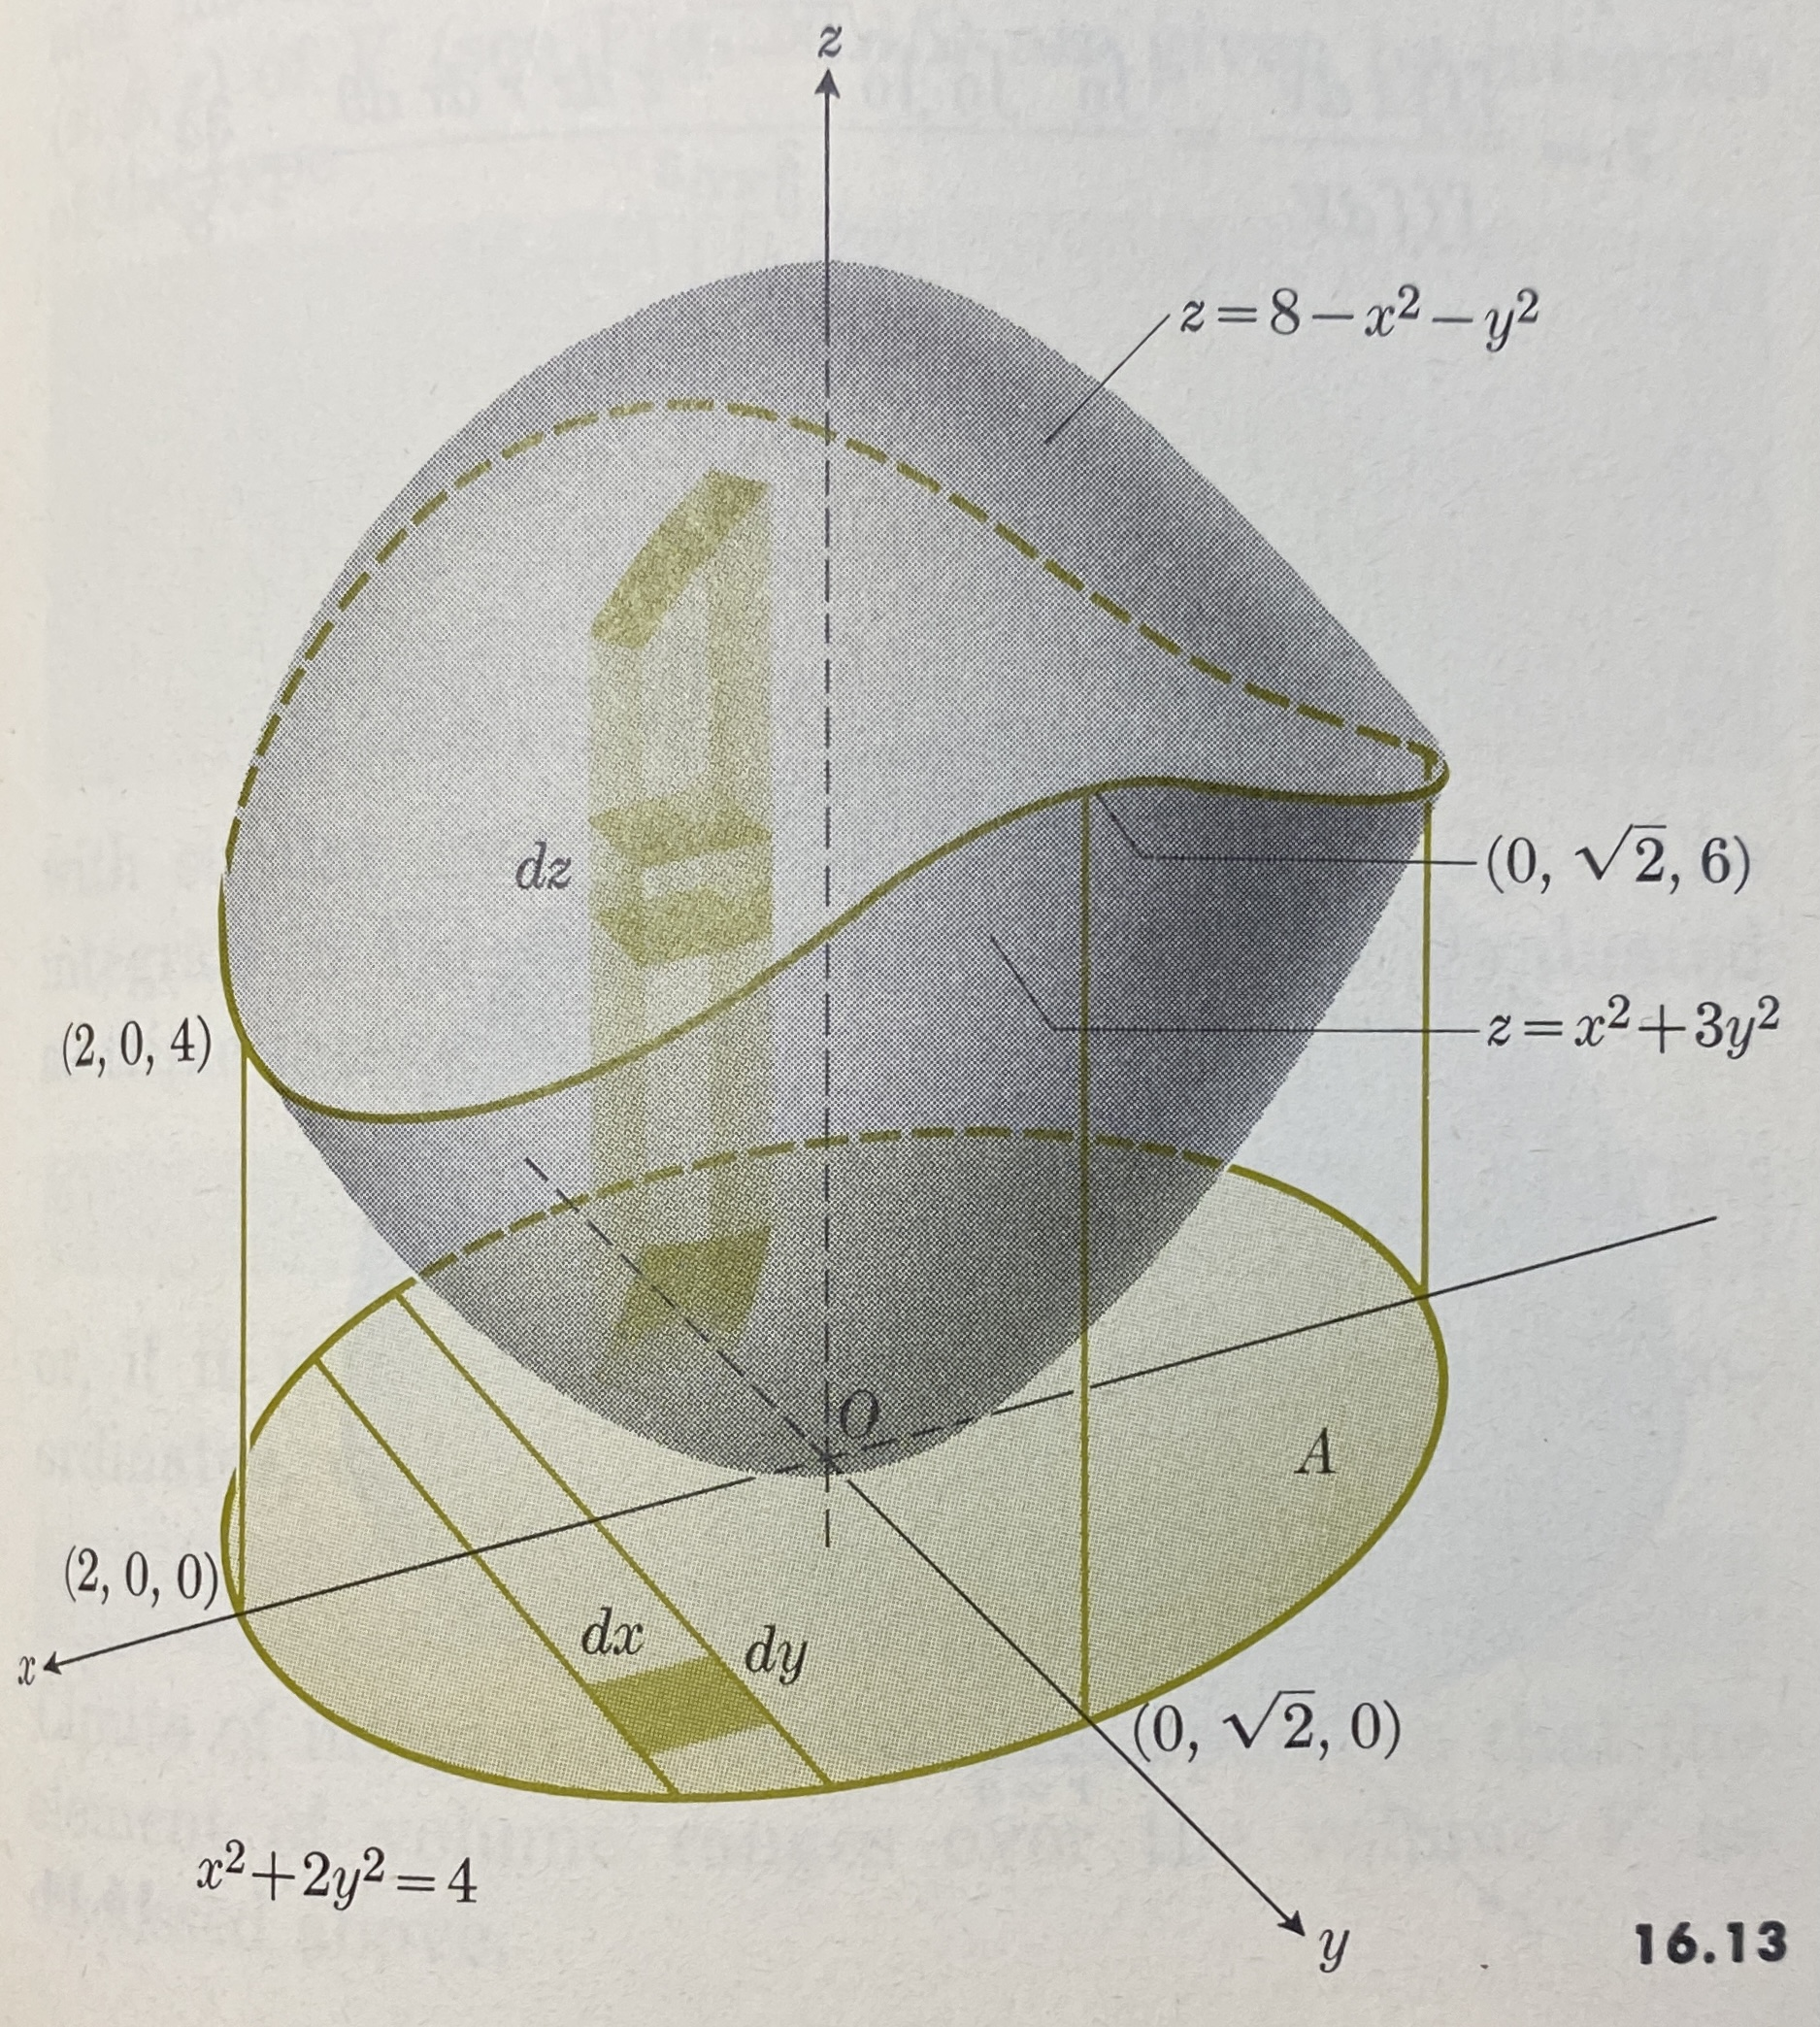
\includegraphics[width=0.4\linewidth]{ExtFiles/volume3Integral.jpg}
        \caption{Volume by triple integration.}
        \label{fig:volume3Integral}
    \end{figure}
    \begin{itemize}
        \item By eliminating $z$ in the two given equations, we can find the elliptic cylinder enclosing $V$ laterally.
        \begin{align*}
            8-x^2-y^2 &= x^2+3y^2\\
            x^2+2y^2 &= 4
        \end{align*}
        \item Thus, to find volume, we evaluate the integral\footnote{One good way to think about this integral is as dividing $V$ up into cross sections parallel to the $yz$-plane at each $x_0\in[-2,2]$, taking the double integral of $F(x_0,y,z)$ over this cross section, and then summing (integrating) all of these cross sections.}
        \begin{equation*}
            V = \int_{-2}^2\int_{-\sqrt{(4-x^2)/2}}^{\sqrt{(4-x^2)/2}}\int_{x^2+3y^2}^{8-x^2-y^2}\dd{z}\dd{y}\dd{x} = 8\pi\sqrt{2}
        \end{equation*}
    \end{itemize}
\end{itemize}



\section{Cylindrical Coordinates}
\begin{itemize}
    \item \dq{Instead of using an element of volume $\dd{V}_{xyz}=\dd{z}\dd{y}\dd{x}$ as we have done, we may use an element $\dd{V}_{r\theta z}=\dd{z}\, r\dd{r}\dd{\theta}$}{560}
    \item Cylindrical coordinates $r,\theta,z$ are particularly useful in problems with an axis of radial symmetry, which we can make to be the $z$-axis.
    \item \dq{Find the center of gravity of a homogenous solid hemisphere of radius $a$}{560}
    \begin{figure}[h!]
        \centering
        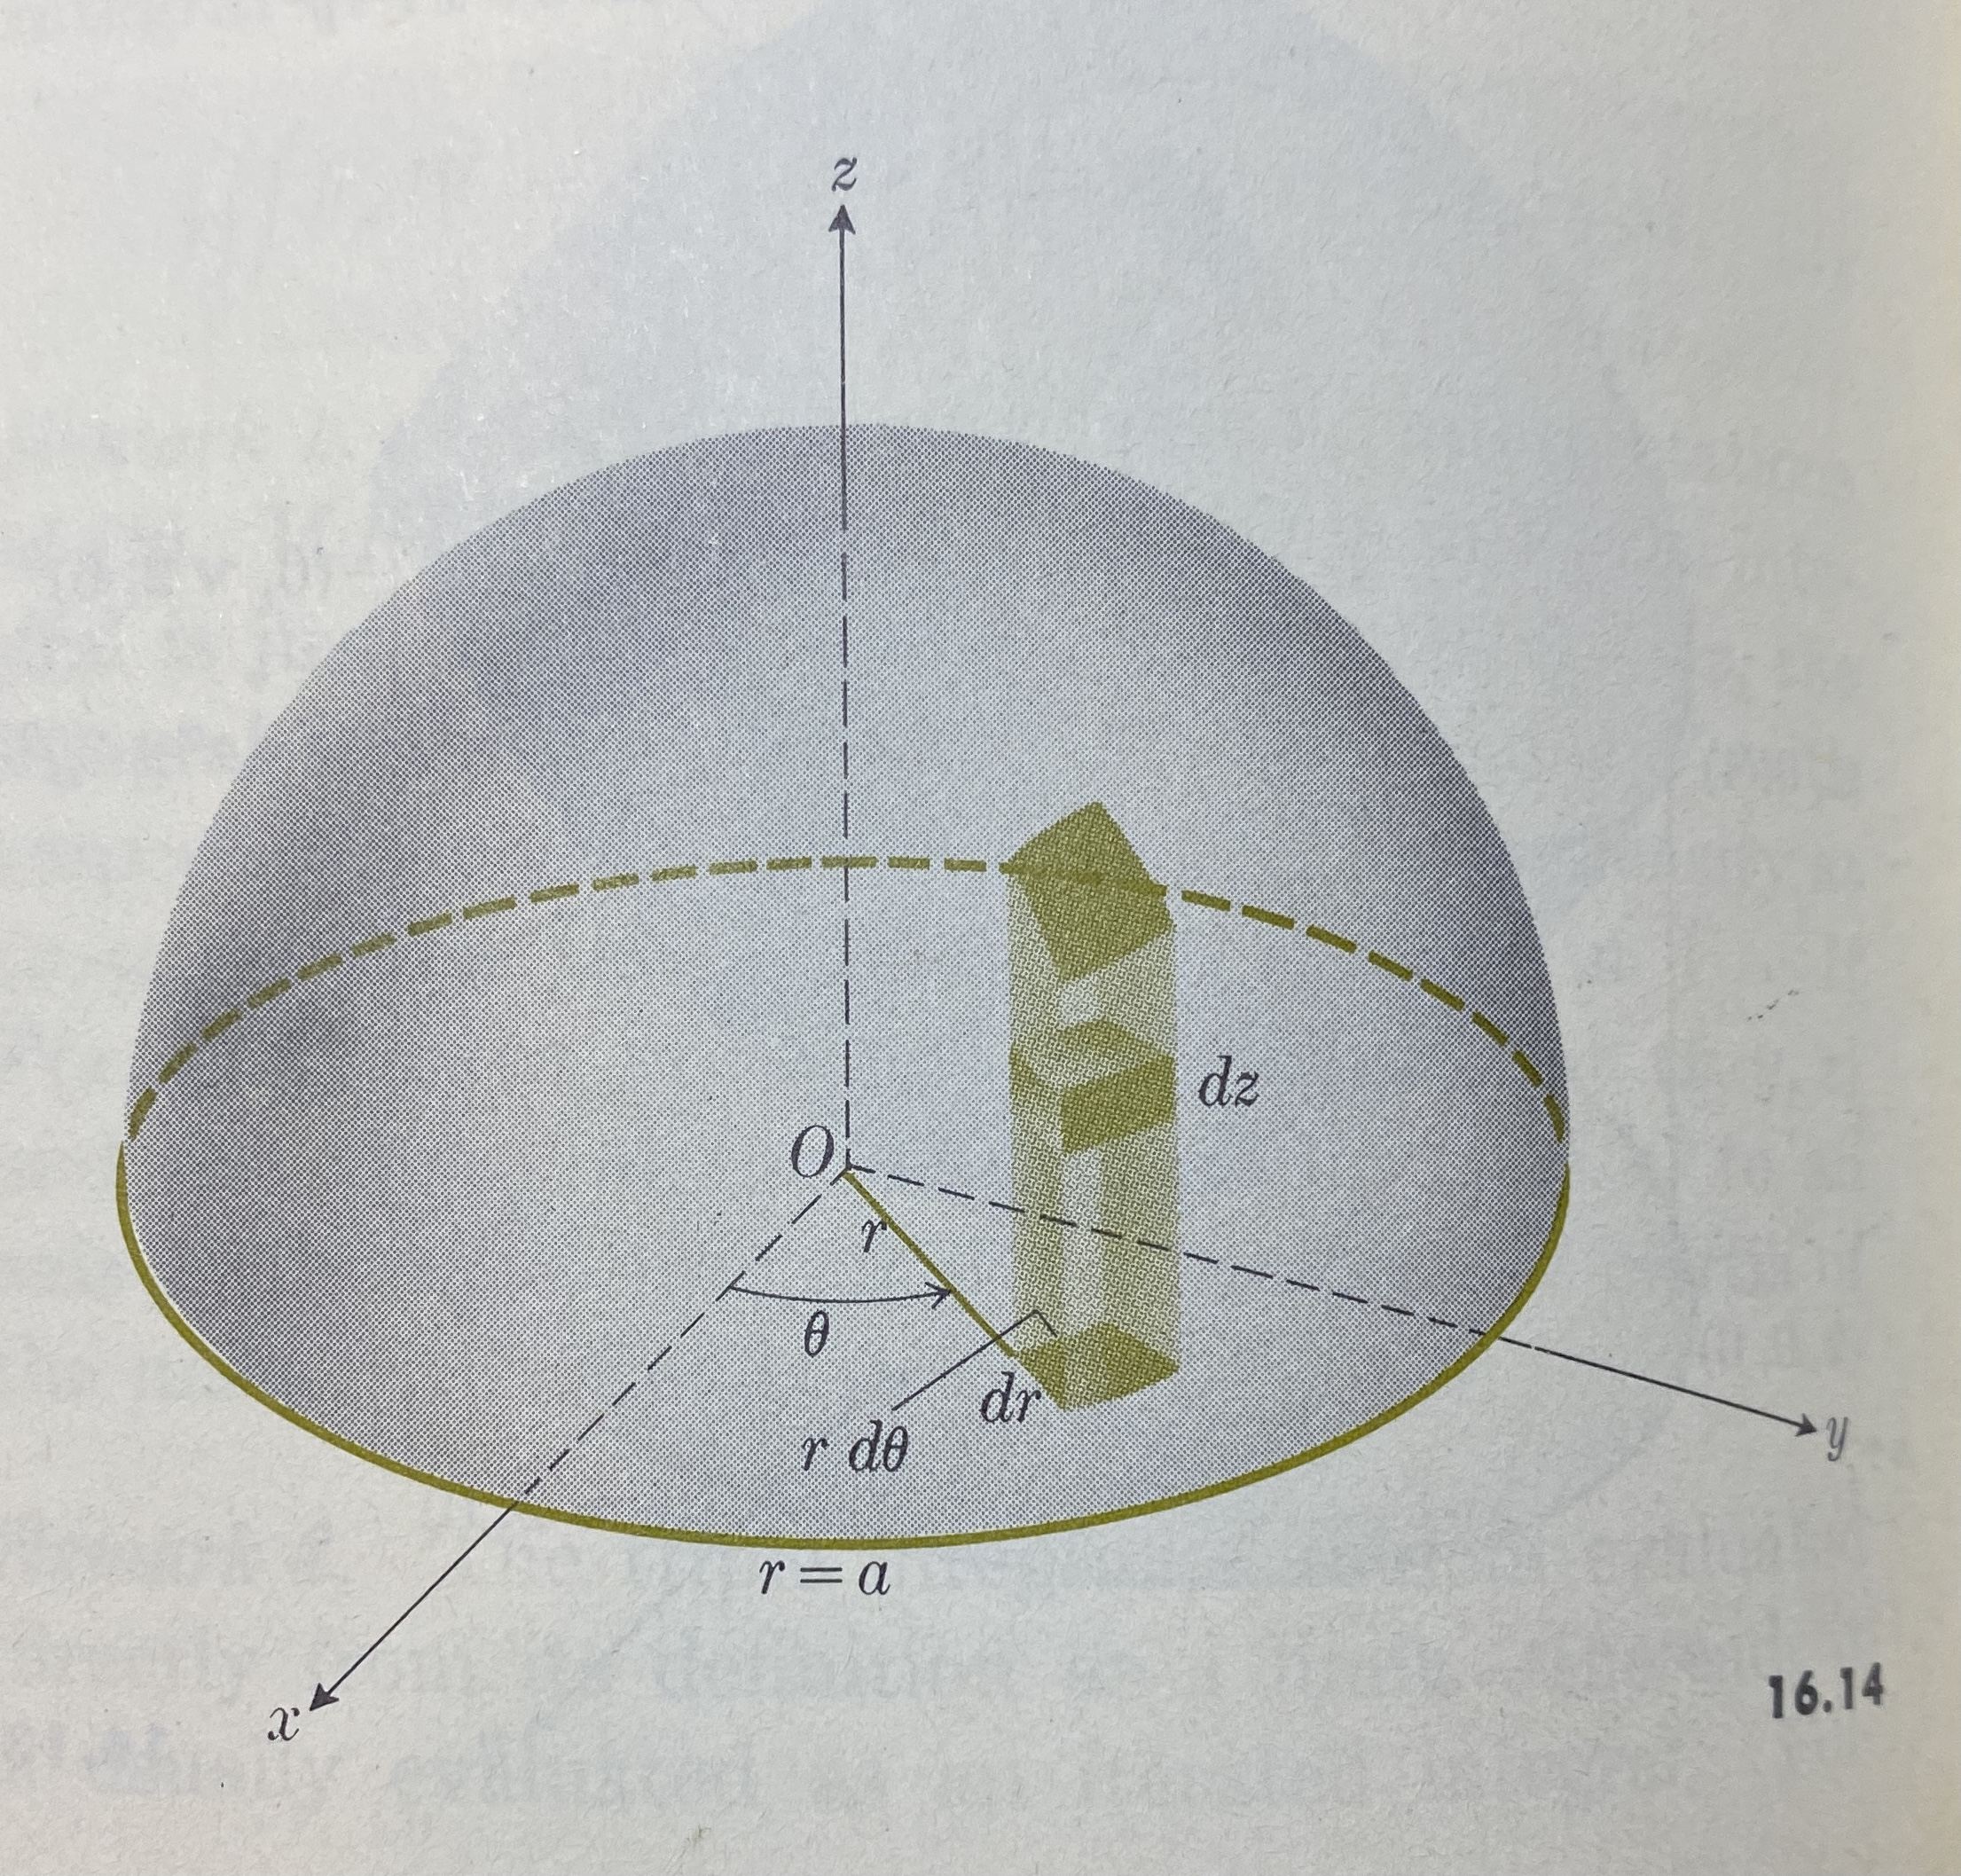
\includegraphics[width=0.4\linewidth]{ExtFiles/hemisphereCOM.jpg}
        \caption{Center of mass of a hemisphere by triple integration.}
        \label{fig:hemisphereCOM}
    \end{figure}
    \begin{itemize}
        \item We let the base of the hemisphere rest on the $xy$-plane so that it exhibits radial symmetry about the $z$-axis, as in Figure \ref{fig:hemisphereCOM}.
        \item By symmetry, we have $x_\text{cm}=y_\text{cm}=0$.
        \item As to $z_\text{cm}$, in cylindrical coordinates, the height of the hemisphere above the $xy$-plane is given by $\sqrt{a^2-r^2}$. Thus, we evaluate
        \begin{equation*}
            z_\text{cm} = \frac{\iiint z\dd{V}}{\iiint\dd{V}}
            = \frac{\int_0^{2\pi}\int_0^a\int_0^{\sqrt{a^2-r^2}}z\dd{z}\, r\dd{r}\dd{\theta}}{\frac{2}{3}\pi a^3}
            = \frac{3a}{8}
        \end{equation*}
    \end{itemize}
\end{itemize}



\section{Physical Applications of Triple Integration}
\begin{itemize}
    \item The mass, center of gravity, and moment of inertia of a mass $M$ distributed over a region $V$ of $xyz$-space with density $\delta(x,y,z)$ at the point $(x,y,z)$ are, respectively,
    \begin{align*}
        M &= \iiint\delta\dd{V}&
            x_\text{cm} &= \frac{\iiint x\, \delta\dd{V}}{\iiint\delta\dd{V}}&
                I_z &= \iiint(x^2+y^2)\, \delta\dd{V}
    \end{align*}
\end{itemize}



\section{Spherical Coordinates}
\begin{itemize}
    \item Spherical coordinates $\rho,\phi,\theta$ are particularly useful in problems with symmetry about a point, which we can make the origin.
    \begin{figure}[h!]
        \centering
        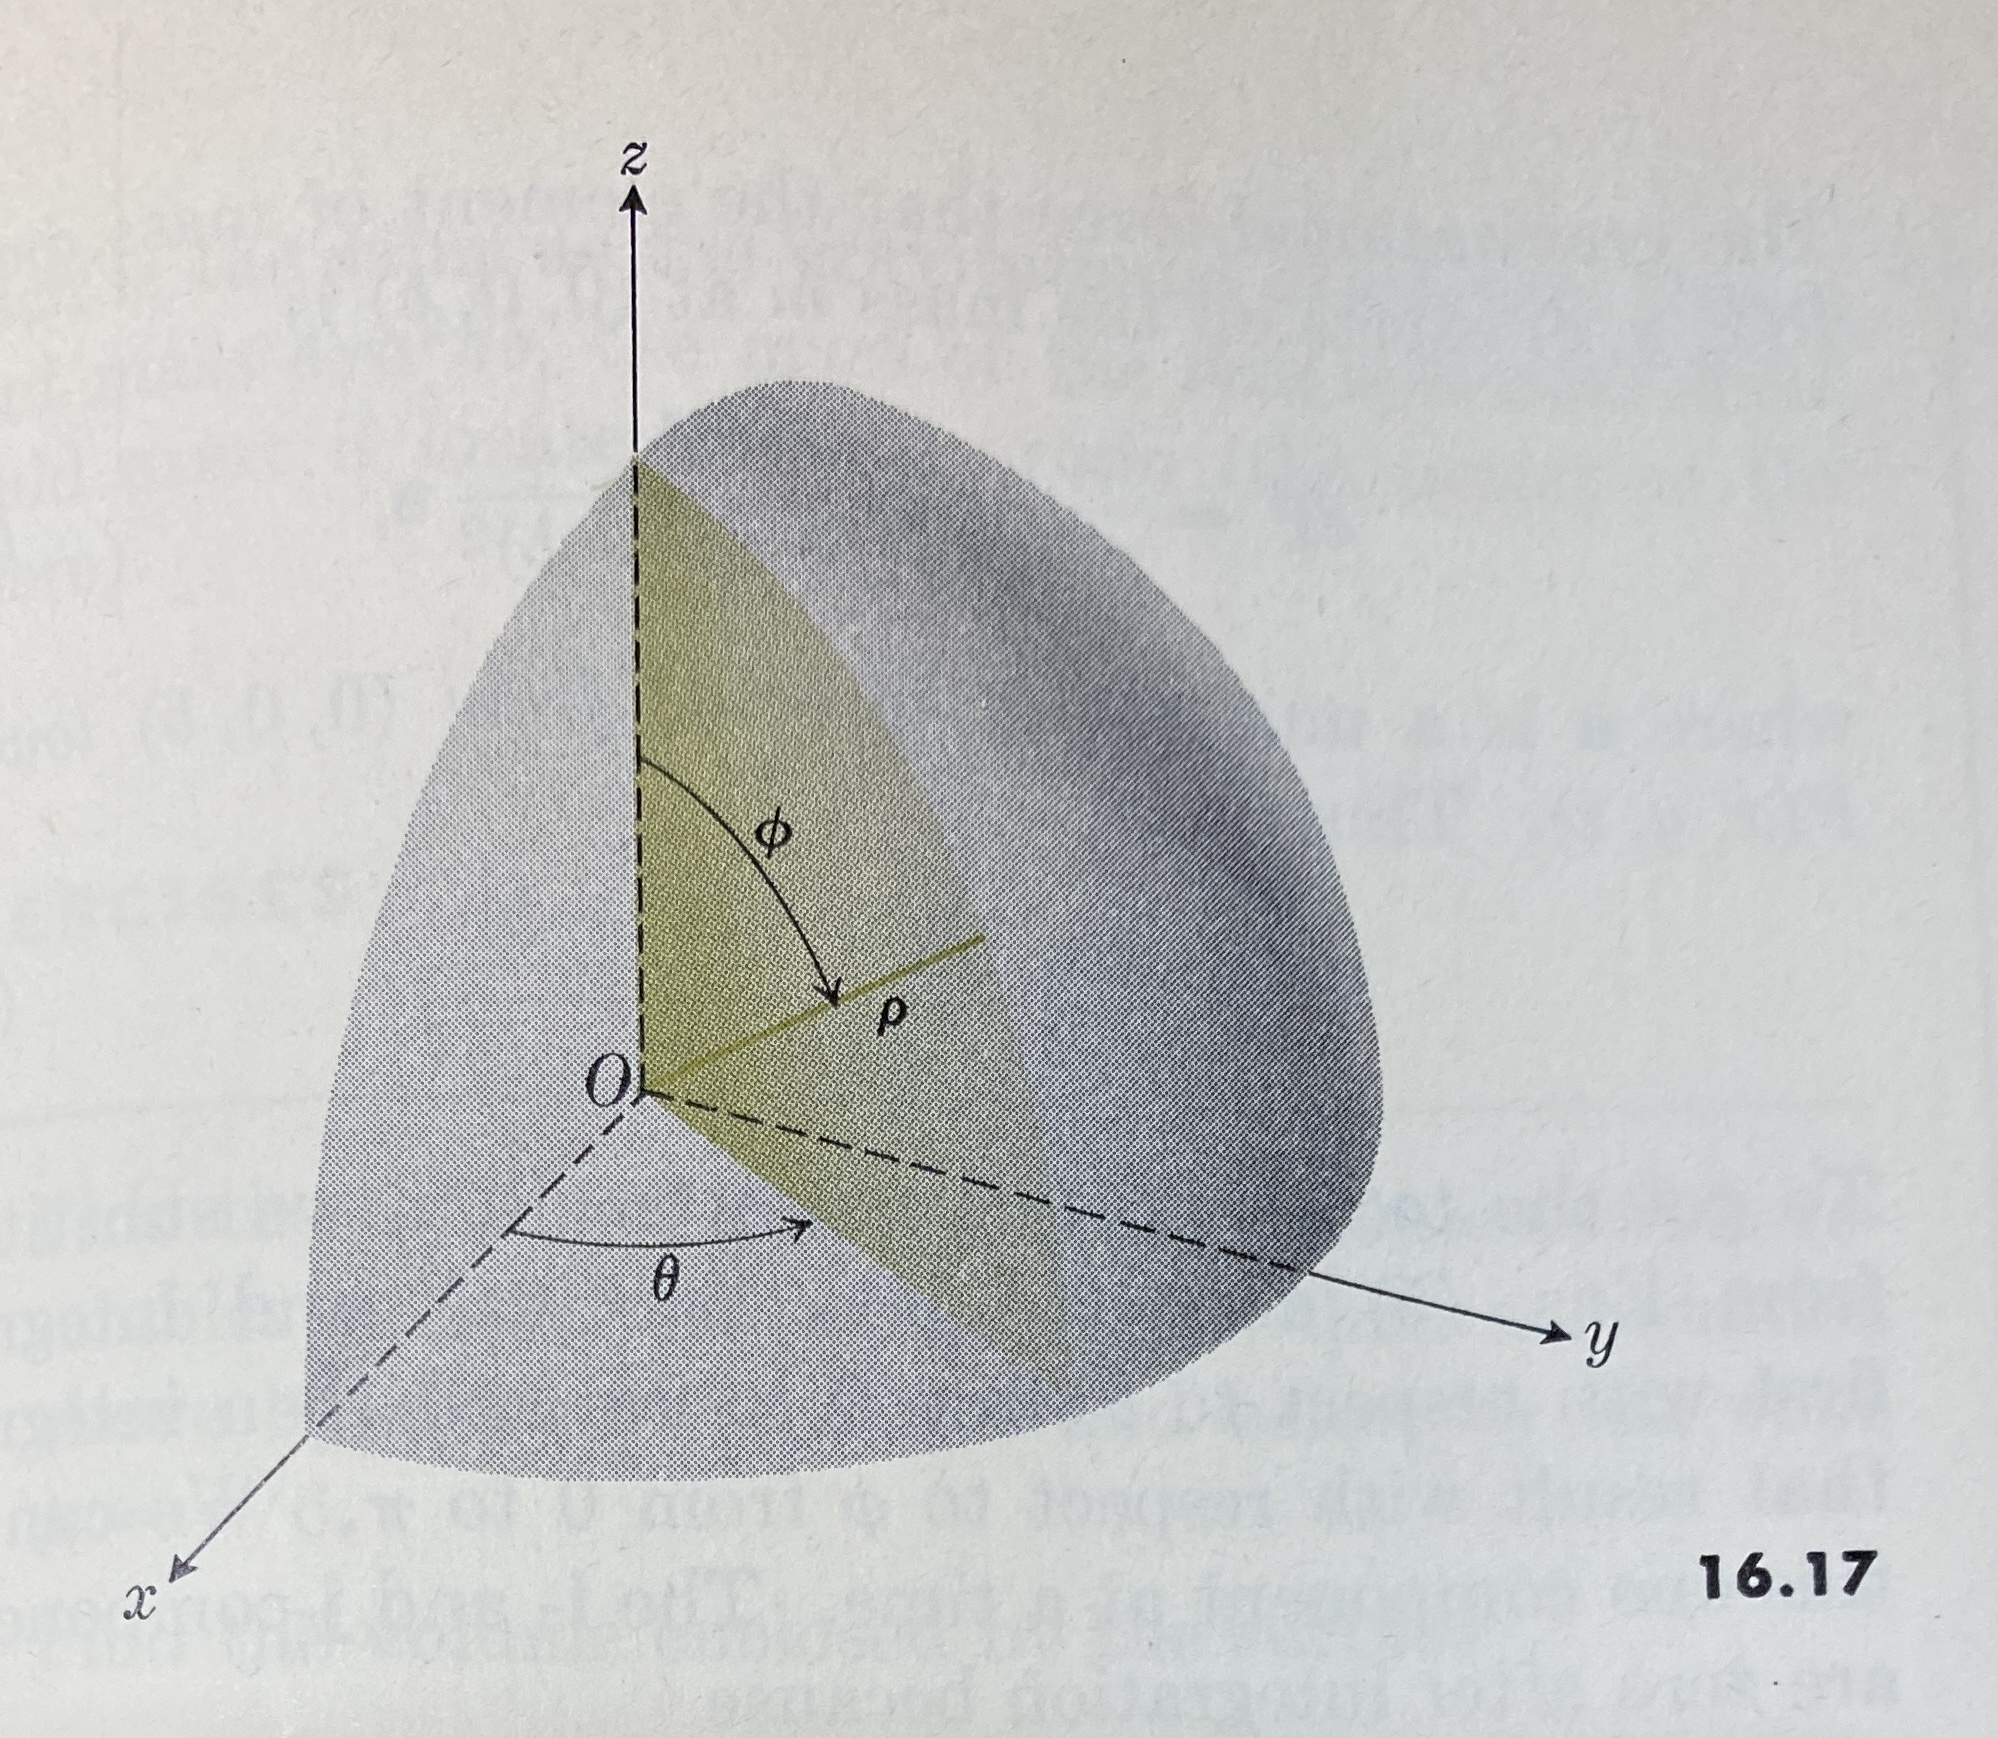
\includegraphics[width=0.4\linewidth]{ExtFiles/sphericalCoordinates.jpg}
        \caption{Spherical coordinates.}
        \label{fig:sphericalCoordinates}
    \end{figure}
    \item We interconvert between spherical and Cartesian coordinates with the equations
    \begin{align*}
        x &= \rho\sin\phi\cos\theta&
            y &= \rho\sin\phi\sin\theta&
                z &= \rho\cos\phi
    \end{align*}
    \item Here, we substitute a volume element $\dd{V}_{xyz}$ for a volume element
    \begin{align*}
        \dd{V}_{\rho\phi\theta} &= \dd{\rho}\cdot\rho\dd{\phi}\cdot\rho\sin\phi\dd{\theta}\\
        &= \rho^2\sin\phi\dd{\rho}\dd{\phi}\dd{\theta}
    \end{align*}
    \begin{figure}[h!]
        \centering
        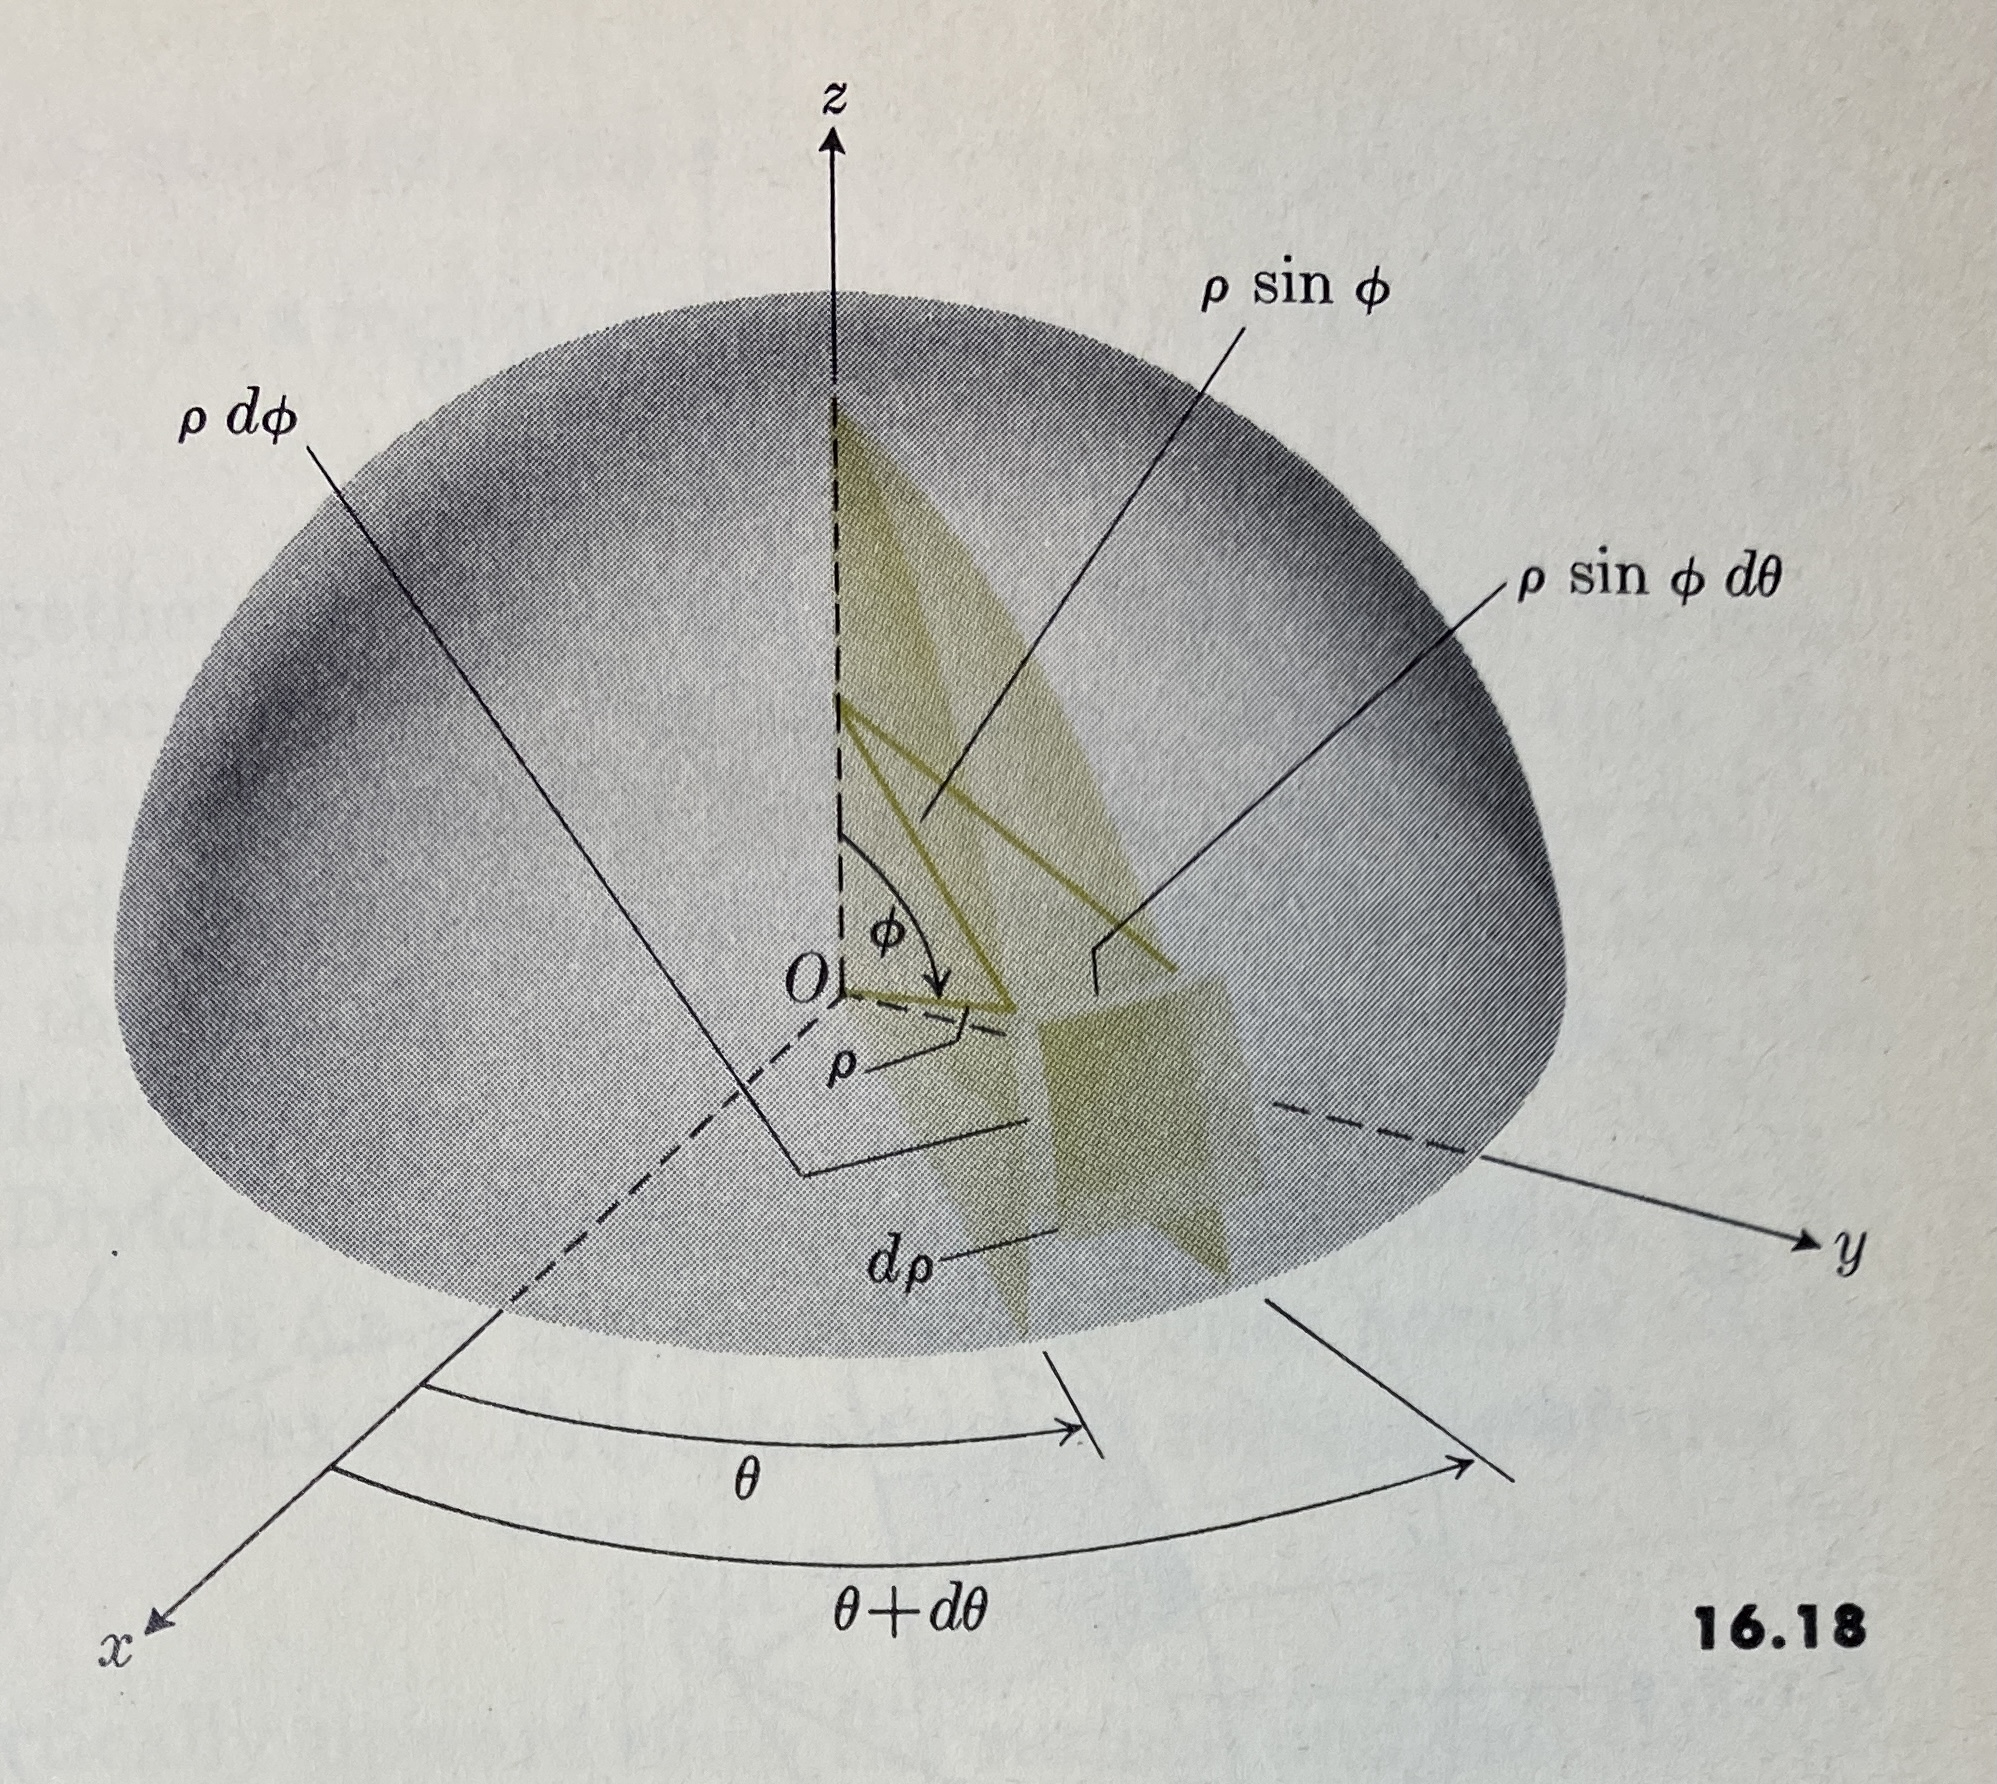
\includegraphics[width=0.4\linewidth]{ExtFiles/dVspherical.jpg}
        \caption{Infinitesimal volume element of spherical coordinates.}
        \label{fig:dVspherical}
    \end{figure}
    \begin{itemize}
        \item Figure \ref{fig:dVspherical} visually justifies the choice of these lengths.
    \end{itemize}
    \item \cite{bib:Thomas} proves that the gravitational attraction of a planet is the same as a point particle of identical mass located at the planet's center.
\end{itemize}



\section{Surface Area}
\begin{itemize}
    \item If $G$ is a region of the $xy$-plane in which $z=f(x,y)$ and its first partial derivatives are continuous, then we can find the surface area of the surface $S$ defined by $f(x,y)$ lying over $G$.
    \begin{figure}[h!]
        \centering
        \begin{subfigure}[b]{0.4\linewidth}
            \centering
            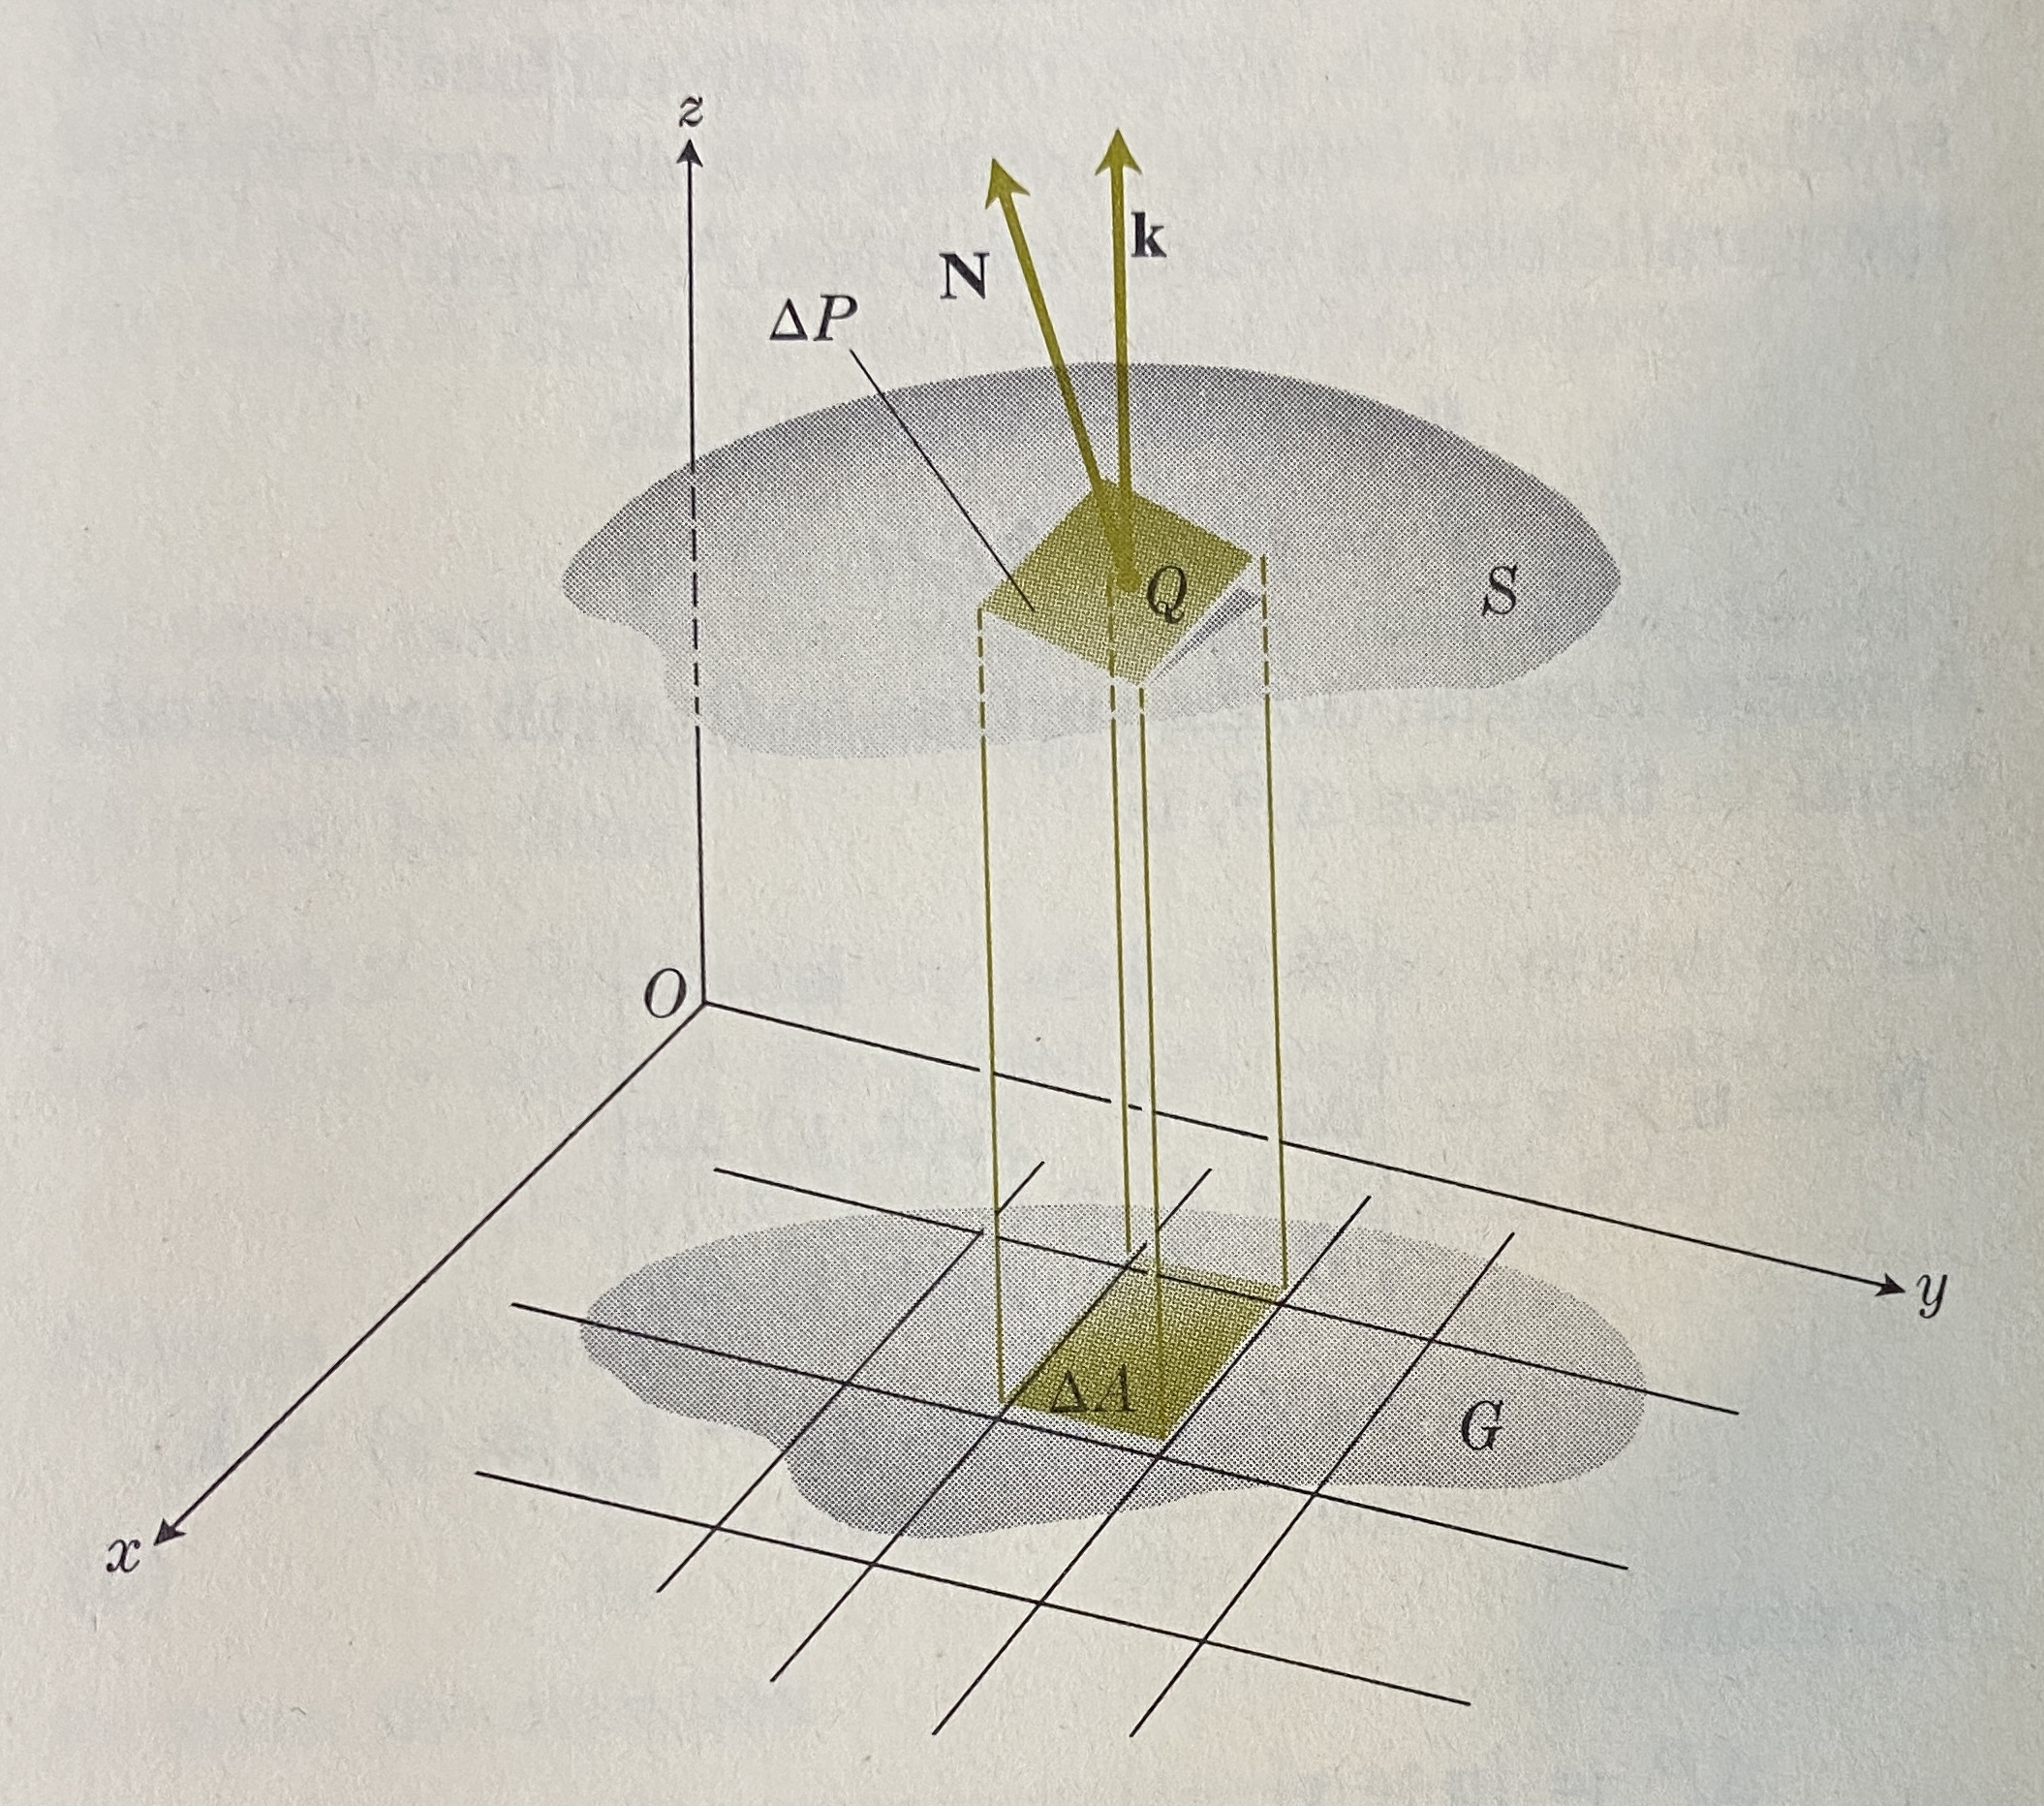
\includegraphics[width=0.9\linewidth]{ExtFiles/surfaceAreaa.jpg}
            \caption{Analyzing the surface.}
            \label{fig:surfaceAreaa}
        \end{subfigure}
        \begin{subfigure}[b]{0.4\linewidth}
            \centering
            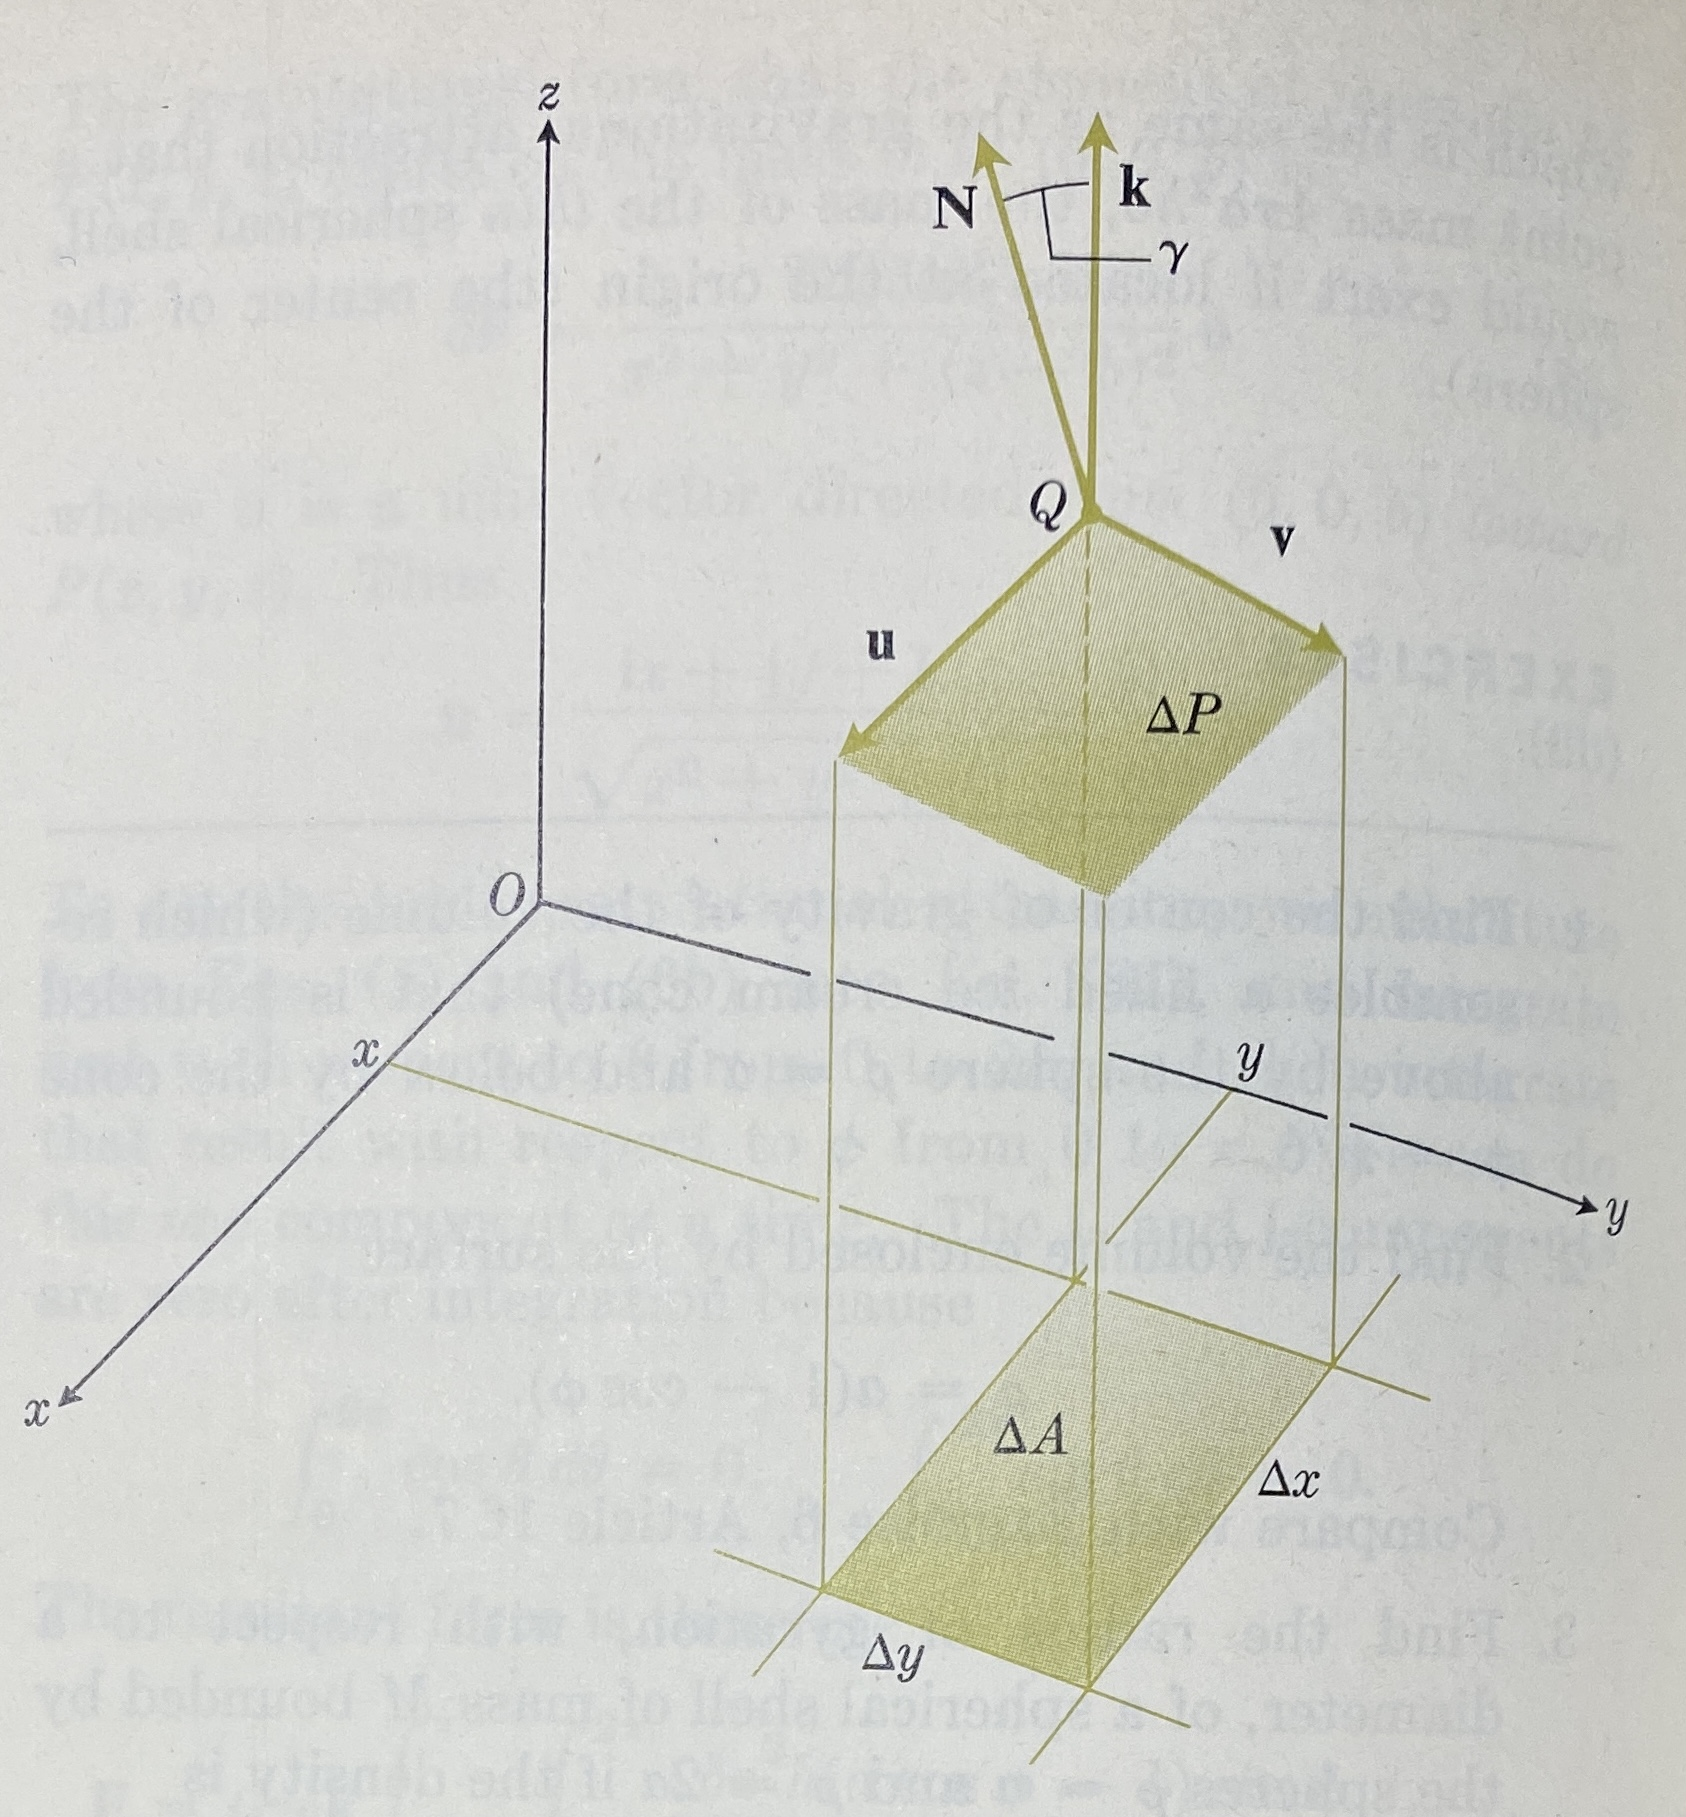
\includegraphics[width=0.9\linewidth]{ExtFiles/surfaceAreab.jpg}
            \caption{Analyzing the approximation.}
            \label{fig:surfaceAreab}
        \end{subfigure}
        \caption{Surface area of a surface defined by a function of two variables.}
        \label{fig:surfaceArea}
    \end{figure}
    \begin{itemize}
        \item We begin by dividing $G$ into rectangles parallel to the $xy$-axes as in Figure \ref{fig:surfaceAreaa}.
        \item Consider one such rectangle $\Delta A$ whose four vertices are $(x,y,0)$, $(x+\Delta x,y,0)$, $(x,y+\Delta y,0)$, and $(x+\Delta x,y+\Delta y,0)$, and let $Q(x,y,f(x,y))$ be the point above $(x,y,0)$ on $S$. We are going to approximate the area $\Delta S$ of the part of $S$ above $\Delta A$ with the area $\Delta P$ of the tangent plane to $Q$ above $\Delta A$.
        \item We can define two vectors $\vb{u}$ and $\vb{v}$ that lie along two of the edges of $\Delta P$, as in Figure \ref{fig:surfaceAreab}, as follows.
        \begin{align*}
            \vb{u} &= \vb{i}\Delta x+\vb{k}f_x(x,y)\Delta x&
                \vb{v} &= \vb{j}\Delta y+\vb{k}f_y(x,y)\Delta y
        \end{align*}
        \item The cross product of these vectors gives both a normal vector $\vb{N}$ to $P$ (and to $S$ at $Q$), and the area of $\Delta P$ (via its magnitude).
        \begin{align*}
            \vb{N} &= \vb{u}\times\vb{v}&
                \Delta P &= |\vb{u}\times\vb{v}|\\
            &= \Delta x\, \Delta y(-\vb{i}f_x(x,y)-\vb{j}f_y(x,y)+\vb{k})&
                &= \Delta x\, \Delta y\sqrt{f_x^2(x,y)+f_y^2(x,y)+1}
        \end{align*}
        \item Now that we have an analytical formula for $\Delta P$, we know that the surface area of $S$ is given by\footnote{It makes sense that this formula is similar to the single-variable calculus arc length formula since surface area is analogous to arc length, just one dimension higher.}
        \begin{equation*}
            SA = \lim_{\Delta x,\Delta y\to 0}\sum_G\Delta P
            = \int_G\int\sqrt{\left( \pdv{f}{x} \right)^2+\left( \pdv{f}{y} \right)^2+1}\dd{x}\dd{y}
        \end{equation*}
    \end{itemize}
    \item Since $(\vb{u}\times\vb{v})\cdot\vb{k}$ is equal to the area of the projection of $\Delta P$ in the $xy$-plane (this can be confirmed by the fact that $[\Delta x\, \Delta y(-\vb{i}f_x(x,y)-\vb{j}f_y(x,y)+\vb{k})]\cdot\vb{k}=\Delta x\, \Delta y=\Delta A$), and since $(\vb{u}\times\vb{v})\cdot\vb{k}=|\vb{u}\times\vb{v}|\, |\vb{k}|\cos\gamma=\Delta P\cos\gamma$, we know that $\Delta P=\Delta A/\cos\gamma$, meaning that
    \begin{equation*}
        SA = \lim_{\Delta x,\Delta y\to 0}\sum_G\Delta P
        = \int_G\int\frac{\dd{A}}{\cos\gamma}
    \end{equation*}
    \begin{itemize}
        \item If the equation of $S$ is given in the form $F(x,y,z)=0$, then $\vb{N}=\nabla F$ and $\cos\gamma=\vb{N}\cdot\vb{k}/(|\vb{N}|\cdot|\vb{k}|)$
    \end{itemize}
    \item Discusses numerical approximations of the surface area integral.
\end{itemize}




\end{document}